% %\documentclass{article} % For LaTeX2e
% \documentclass[conference,10pt]{IEEEtran}
% %\usepackage{nips14submit_e,times}
% 
% \usepackage[sc]{mathpazo}
% %\linespread{1.05}         % Palatino needs more leading (space between lines)
% \usepackage[T1]{fontenc}
% 
% \usepackage{url}
% %\documentstyle[nips13submit_09,times,art10]{article} % For LaTeX 2.09
% 
% \usepackage{hyperref}
% \usepackage[usenames,dvipsnames]{color}
% \definecolor{orange}{rgb}{0.8,0.4,0}
% \definecolor{mylink}{RGB}{18,68,115}
% \definecolor{darkgreen}{rgb}{0.3,0.6,0.3}
% 
% \usepackage{graphicx}
% %\usepackage[footnotesize]{caption}
% \usepackage[numbers,sort&compress]{natbib}
% 
% \hypersetup{letterpaper,bookmarksopen,bookmarksnumbered,
% pdfpagemode=UseOutlines,
% colorlinks=true,
% linkcolor=mylink,
% anchorcolor=blue,
% citecolor=mylink,
% filecolor=blue,
% menucolor=blue,
% urlcolor=mylink,
% }
% %\usepackage{multicol}
%  
% % Labels in IEEE format
% % Equation
% \newcommand{\eref}[1]{Eq.(\ref{#1})}
% % Figure
% \newcommand{\figref}[1]{Fig.\ref{#1}}
% 
% \usepackage{ifthen}
% 
% \newboolean{include-notes}
% \setboolean{include-notes}{true}
% % http://en.wikibooks.org/wiki/LaTeX/Colors
% \newcommand{\ssnote}[1]{\ifthenelse{\boolean{include-notes}}%
%  {\textcolor{orange}{\textbf{SS: #1}}}{}}
% \newcommand{\adnote}[1]{\ifthenelse{\boolean{include-notes}}%
%  {\textcolor{LimeGreen}{\textbf{AD: #1}}}{}}
% 
% \usepackage[font=footnotesize]{caption}
% \usepackage{subcaption}
% 
% \title{\Large Chisel: Real-time Dense Reconstruction on a Mobile Device \\
% using Spatially Hashed Truncated Signed Distance Fields \\
% REVIEW COPY}
% 
% \newcommand{\fix}{\marginpar{FIX}}
% \newcommand{\new}{\marginpar{NEW}}
% 
% %\nipsfinalcopy % Uncomment for camera-ready version
% \usepackage{amsmath,amssymb,amsthm}
% \begin{document}
% 
% \author
% {
% Authors omitted for review.
% 	%Matthew Klingensmith \\
% 	%Carnegie Mellon Robotics Institute\\
% 	%\texttt{mklingen@andrew.cmu.edu}
% 	%\and
% 	%Ivan Dryanovski \\
% 	%City College of New York\\
% 	%\texttt{ivan.dryanovski@gmail.com}
% }
% 
% 
% \maketitle
\documentclass[10pt,twocolumn,letterpaper]{article}

\usepackage{cvpr}
\usepackage{times}
\usepackage{epsfig}
\usepackage{graphicx}
\usepackage{amsmath}
\usepackage{amssymb}
\usepackage[font=footnotesize]{caption}
\usepackage{subcaption} 

% Include other packages here, before hyperref.

% If you comment hyperref and then uncomment it, you should delete
% egpaper.aux before re-running latex.  (Or just hit 'q' on the first latex
% run, let it finish, and you should be clear).
\usepackage[pagebackref=true,breaklinks=true,letterpaper=true,colorlinks,bookmarks=false]{hyperref}

 \cvprfinalcopy % *** Uncomment this line for the final submission

\def\cvprPaperID{****} % *** Enter the CVPR Paper ID here
\def\httilde{\mbox{\tt\raisebox{-.5ex}{\symbol{126}}}}

% Pages are numbered in submission mode, and unnumbered in camera-ready
\ifcvprfinal\pagestyle{empty}\fi
\begin{document} 

%%%%%%%%% TITLE
\title{\Large Chisel: Real-time Dense Reconstruction on a Mobile Device \\
using Spatially Hashed Truncated Signed Distance Fields}

\newcommand{\fix}{\marginpar{FIX}}
\newcommand{\new}{\marginpar{NEW}}

%\nipsfinalcopy % Uncomment for camera-ready version
\usepackage{amsmath,amssymb,amsthm}
\begin{document}

\author
{
	Matthew Klingensmith \\
	Carnegie Mellon Robotics Institute\\
	\texttt{mklingen@andrew.cmu.edu}
	\and
	Ivan Dryanovski \\
	The Graduate Center,\\
	City University of New York\\
	\texttt{idryanovski@gc.cuny.edu}
}

\maketitle
%\thispagestyle{empty}
\begin{figure}
  \centering
    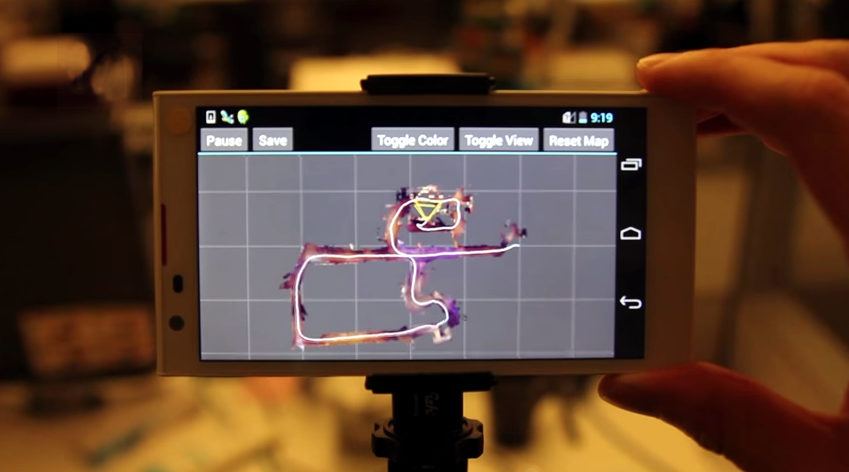
\includegraphics[width=1.0\columnwidth]{img/mapdevice}
      \caption{Our algorithm recording a map of an office building floor on a mobile
  device in real time, at a resolution of 3cm. A video of our approach running
  in real time can be found here: \cite{TangoVideo}.}
  \label{fig:map_device}
\end{figure}


\begin{abstract}
Google's project \textit{Tango}\cite{Tango} has made depth sensing available to
mobile devices such as phones and tablets. Because these devices have limited
computing power, memory, and graphics capabilities, doing real-time 3D
reconstruction with them remains challenging. Existing approaches are either too
inefficient for use on mobile devices, or only consider sparse reconstructions.
We propose an efficient method of real-time dense 3D reconstruction using
chunked, dynamic spatial hash maps \cite{SpatialHashing} of truncated signed
distance volumes \cite{Curless1996}. We show that our method is able to
reconstruct and render very large scenes in real time using only the phone's
CPU and the fixed function graphics pipeline, with a minimal memory footprint
in comparison to existing approaches. We provide both qualitative and
quantitative results on publicly available RGB-D datasets \cite{FREIBURG}, and
on datasets collected in real-time from two devices.
\end{abstract}

\section{Introduction}
% \begin{itemize}
%     \item We want to do large-scale 3D reconstruction from depth data with only
%     limited hardware.
%     \item This is attractive for many use cases where all one wants to do is
%     make a rough mesh of an area. The real-time aspect allows the user to see
%     the accuracy of the reconstruction easily. This is also attractive for small
%     mobile robots (such as quad-copters) with limited onboard compute power.
%     \item We have access to VIO, and so don't need to do pose estimation
%     \item Existing techniques are not sufficient for the amount of compute power
%     we have
%     \item We want to be careful about maintaining probabalistically accurate
%     data and not throwing it away/compressing it.
%     \item It's important to keep track of the noise model of the sensor to deal
%     with noise, distortion and missing data.
%     \item We want to use the TSDF over occupancy grids \cite{Elfes1989} or
%     octomaps \cite{Wurm2010}, because the TSDF is much better at maintaining
%     surface information, and occupancy information can easily be extracted from
%     it.
%     \item We also want to use the color camera, but don't want to make a
%     photometrically accurate model due to our limited compute power.
% \end{itemize}

Mobile devices are beginning to offer a wide range of sensors normally found on
robots: gyroscopes, accelerometers, compasses, GPS units, and high resolution
sensors are now common place in average market phones. Recently, mobile phone
manufacturers have expressed interest in using depth sensors in mobile devices;
this opens up interesting possibilities for 3D reconstruction, mapping,
and object recognition on such devices that were previously unavailable. In
particular, the devices we use in this work, Google's Tango \cite{Tango} phone
and tablet use a small active ifrared projection depth sensor combined with
high-performance IMUs and a wide field of view camera. Mobile devices with depth
sensors also provide an attractive, light-weight, integrated platform for small mobile robots.

We are interested in the problem of real-time 3D reconstruction. The task is to
extract the true 3D geometry and color of a real scene from a sequence of noisy
sensor readings. Solutions to this problem are useful for mobile robot navigation,
indoor localization, mapping, and object scanning. The problem is ill-posed,
since it requires localization as well as mapping (and hence is a variant of
the SLAM problem.)

Real-time 3D reconstruction remains challenging on mobile devices. Compared to
full-sized machines, mobile devices have severely limited processing power,
memory requirements, and graphics capabilities. Further, the depth sensors
available on these devices are much more limited than their full-sized
counterparts; they are typically lower resolution, have slower refresh rates,
and have much more undesirable nonlinear distortion and noise.

Previous work on high quality real-time 3D reconstruction \cite{Newcombe,
Whelan2013, Bylow2013, DTAM} has focused on much more capable and high-powered
computing platforms with much more accurate sensing, and is therefore not well
suited for low-powered mobile devices. At the same time, works which perform 3D
reconstruction on mobile phones have either relied on low quality sparse
keypoint-based methods \cite{KleinSparse}, or else require intensive offline
computation \cite{TanskanenMetric} for dense 3D mapping.

In this work, we propose a novel algorithm for efficient real-time 3D
reconstruction on mobile devices with onboard depth sensors. We show that even
with a low-powered mobile device with severe limitations on memory usage,
processing power, and graphics capabilities, relatively high-quality,
large-scale real-time 3D reconstruction is feasible. Our algorithm relies on
using a dynamic spatial hash map \cite{SpatialHashing} to directly store
distance field data, which greatly reduces the amount of memory required to
store the reconstruction as compared to state of the art approaches.

\section{Related Work}
% \begin{itemize}
%     \item Real-time mapping solutions started with occupancy grids
%     \cite{Elfes1989}. But implemented in a naive way, these are too memory
%     intensive for our purposes. They are also bad at surface reconstruction.
%     \item More recent work in occupancy grid mapping reduces their memory
%     footprint by introducing an octree structure \cite{Wurm2010}. However,
%     octree structures have a hefty lookup time for each access, read, or write.
%     They also have poor cache performance during iteration.
%     \item \cite{Curless1996} introduced the TSDF as an efficient, accurate way
%     of reconstructing surfaces from many registered depth images. These are more
%     desirable for surface reconstruction than occupancy grids, because they
%     maintain local structure (inside vs. outside).
%     \item \cite{Newcombe}, introduced a method (Kinect Fusion) of creating and
%     registering TSDF volumes to depth images in real-time using ICP-like alignment of scans.
%     Making heavy use of GPU computing, Kinect fusion is able to generate and
%     display extremely high-quality reconstructions in a small area (due to
%     using a fixed size volume for reconstruction). 
%     \item Attempting to increase the size of Kinect Fusion reconstructions and
%     reduce drift, Kintinuous \cite{Whelan2013} keeps a running window of the
%     scene that gets integrated into a TSDF. Parts of the scene outside the
%     window are turned into a mesh with simple greedy triangulation. While this
%     allows them to make larger reconstructions than Kinect Fusion, they lose
%     distance field data as they move around the scene -- data which might still
%     be useful in its uncompressed form. We want to do large-scale reconstruction
%     \emph{without} compressing volumetric data into a surface representation
%     first.
%     \item Like \cite{Whelan2013}, \cite{Bylow2013} use the volume structure
%     directly to store colors. We copy the method of \cite{Bylow2013} to colorize
%     our meshes due to the simplicity and speed of the method.
% \end{itemize}
Real-time mapping and localization has long been a research topic in robotics
and computer vision. Mapping paradigms generally fall into one of two
categories: landmark-based (or \emph{sparse}) mapping, and high-resolution
\emph{dense} mapping. The distinction between the two is that sparse mapping
generates a metrically consistent map of landmarks based on key features in the
environment, while dense mapping globally registers all sensor data into a
high-resolution data structure. In this work, we are concerned primarily with
dense mapping, as at least some components of dense mapping are needed for high
quality 3D reconstruction. 

One of the simplest means of dense 3D reconstruction is to  store a \emph{Point
Cloud} of the scene. This is done by projecting depth images into the scene as
points, and then aligning point clouds to the existing scene; this is done
either through a local pairwise registrion procedure, or a global optimization
procedure. While simple, point clouds fail to capture local scene structure, are highly 
redundant, noisy, and memory intensive.  Additionally, point clouds fail to
capture \emph{negative} information about the scene :  \emph{i.e}, determining
which parts of the scene are empty.  This information is crucial in situations
where the sensor is noisy, or has large patches of missing data \cite{Klingensmith2014}.

Elfes \cite{Elfes1989} introduced the concept of \emph{Occupancy Grid
Mapping}, which divides the world into a 2D grid of axis-aligned cells
(\emph{i.e} Voxels), each of which contains an occupancy probability. Occupancy
grids provide a principled alternative to simple point clouds. They preserve local
structure, and gracefully handle redundant and missing data.
Unfortunately, occupancy grids are prohibitively memory intensive in 3D, since
the amount of memory needed to store the grid increases with the cube of distance 
traveled by the sensor. While more robust than point clouds, occupancy grids
suffer from aliasing, and lack information about surface normals and the
interior/exterior of obstacles.

Attempts to extend occupancy grid maps to 3D have sometimes relied on octrees.
Rather than storing a fixed-resolution grid, octrees store occupancy data in a
spatially organized tree. In typical scenes, octrees reduce the required memory
over occupancy grids by orders of magnitude. Octomap \cite{Wurm2010} is a
popular example of the octree paradigm. However, octrees containing only
occupancy probability suffer from many of the same problems as occupancy grids:
they lack information about the interior and exterior of objects, and suffer
from aliasing. Further, octrees suffer from logarithmic reading, writing, and
iteration times, and have very poor memory locality characteristics.

Curless \cite{Curless1996} introduced an alternative to occupancy grids for 3D
reconstruction which, instead of storing the occupancy probability for each
voxel, stores an approximation of the signed distance field of the scene. The signed distance
field is a mapping from $\mathbf{R}^3$ to $\mathbf{R}$ which represents the
distance to the nearest surface. The SDF is negative inside obstacles, and
positive outside obstacles. The surface is given implicitly as all points in
space where the value of the SDF is zero. The structure introduced in
\cite{Curless1996} only maintains the distance function within a small distance 
(called the \emph{truncation distance}) from observed surfaces, and thus is called the
Truncated Signed Distance Field (TSDF).  While using more memory than occupancy
grids, the TSDF is much more informative for surface reconstruction, as the
implicit surface normals can be extracted from the gradient of the function,
allowing for a higher quality reconstruction.

The \emph{Kinect Fusion} \cite{Newcombe} algorithm uses a TSDF to
simultanesously extract the pose of a moving depth camera and the geometry of a
scene in real-time. Kinect Fusion solves the real-time 3D reconstruction problem
by using incremental estimates of the TSDF to inform the pose of the camera.
Making heavy use of the GPU for raycasting and rendering, Kinect Fusion is
capable of creating extremely high-quality, high-resolution surface 
reconstructions within a small area. However, like occupancy grid mapping, the
algorithm relies on a single fixed-size 3D grid of voxels, and thus is not
suitable for reconstructing very large scenes. Fusion also suffers from pose
drift as small localization errors accumulate.

The \emph{Kintinuous} \cite{Whelan2013} algorithm extends Kinect Fusion to
larger scenes by storing only a time-limited moving window of the TSDF. As the camera
moves outside of the window, areas which are no longer visible are turned into a
triangular mesh. Like Fusion, Kintinuous relies on very high-performance GPU
computing to create its reconstruction.  By prematurely turning the TSDF into an
explicit surface mesh, Kintinuous throws away past data -- and thus the user
cannot return to an area that was previously explored and update the TSDF there.

Our approach uses a TSDF as in\cite{Curless1996,Newcombe,Whelan2013,Bylow2013},
to store an estimate of the signed distance field of the scene. Unlike Kinect
Fusion, and like Kintinuous, we store a dynamic representation of the TSDF
which grows in size as the sensor travels through space. Unlike Kintinuous, we
do not prematurely throw away distance function data by converting it into a
mesh -- instead, we turn small areas of the scene into meshes for the purpose
of rendering, while preserving the underlying distance field data. In this way,
we extend the TSDF surface reconstruction paradigm to very large scenes when only
very limited compute power is available.

Because mobile phones typically have access only to 2D cameras, previous works
on dense reconstruction for mobile phones have gone to great lengths to extract
depth from a series of registered monocular camera images.  Early works on
real-time reconstruction and navigation on mobile devices relies on a spase
mapping, \cite{KleinSparse}, and is unable to produce dense 3D surface
reconstructions.  A recent algorithm by Tanskanen \emph{et. al.}
\cite{TanskanenMetric} generates impressive 3D reconstructions of small scenes
by means of monocular stereo computation and keypoint tracking. However,
because they \cite{TanskanenMetric} must intensively compute a depth map at
each frame by stereo, each frame capture still takes a few seconds, and only a
point cloud is stored. Another work by Newcombe \emph{et. al.}, \textit{Dense
Tracking and} Mapping (DTAM) \cite{DTAM},  creates extremely high quality,
dense 3D reconstructions of scenes in real time using only a monocular camera
-- while the camera is attached to a high-performance desktop computer. 

It should be noted that since our work focuses on mobile devices with depth
cameras attached, such as the Google \emph{Tango} devices \cite{Tango}, we
luckily do not need to perform costly monocular stereo as a pre-requisite to
dense reconstruction. This allows us to save our memory and CPU buget for the
3D reconstruction itself.

\section{Approach} 
% \begin{itemize}
%     \item We start by getting an accurate probablistic model of the depth error
%     on the sensor by training a quadratic model of the depth and noise per
%     pixel. Depth images are compensated by this model before being passed into
%     our system.
%     \item We get pose by monocular visual-intertial odometry, rather than by
%     directly estimating pose from the depth image.
%     \item Depth comes in at 3-5Hz, as does RGB, but never at the same time.
%     \item Explain the TSDF
%     \item We represent the world as a collection of fixed size 16x16x16
%     \emph{Meta-Voxels} or \emph{Chunks}, aligned next to each other. Chunks are
%     allocated only when rays from the sensor would cause them to be updated.
%     They are garbage collected whenever there is no voxel with no weight in it.
%     \item To update a chunk with depth data, we can do one of two things:
%     \emph{Raycasting}, or \emph{Voxel Projection}. In the raycasting case, we
%     efficiently march rays through voxels in each updated TSDF volume, and
%     update the signed distance and weight there. In the voxel projection case,
%     we project the center of each voxel onto the image, and according to the
%     distance from the center of the voxel as compared with the depth from the
%     sensor, we either add weight to it, carve it, or do nothing to it.
%     \item Raycasting is O(number of rays), while Voxel Projection is O(number
%     of voxels). Voxel projection is an aliased approximation of raycasting. 
%     \item To do color, we project the points along the ray we are updating onto
%     the color image. We then update a separate \emph{Color Chunk} with data from
%     the RGB image.
%     \item We use a dynamic trunction distance based on the sensor model.
%     \item Rendering is handled by incrementally creating meshes of the updated
%     chunks using Marching Cubes. Chunks are frustum culled based on the frustum
%     of the renderer's camera, and only those which are near the camera and
%     inside its frustum are rendered. Faraway chunks are rendered as boxes. This
%     allows us to very efficiently render huge areas using only the fixed
%     function pipeline -- an important feature for devices with limited graphics
%     capability.
% \end{itemize}
\subsection{Depth Data and Noise Model}
\label{subsection:calibration}
We begin by considering the data from the device. We will assume that the device
has a depth sensor attached. The depth sensor produces a depth image, which is
a discrete map containing sensed distances from the scene to the image plane.

Consider an ideal pinhole camera model of the depth sensor. We can cast a ray
from the sensor origin through the image plane to surfaces in the world. The
length of that ray is the resulting depth at that point in the image plane. Call
the point on the image plane that the ray intersects $p$. The length of the ray
through $p$ to the scene is given by $z_p$. 

The depth image may be corrupted by noise, feature nonlinear distortions, and
have large segments of missing data. Our noise model of the sensor will consider
Gaussian noise on the depth, and per-pixel quadratic distortion. Call the depth
 measurement at $p$ the random variable $D_p$. Then,
 
 \begin{equation}
 	D_p = z_p + a_p{z_p}^2 + b_p z_p + c_p + \epsilon(z_p)
 \end{equation} 
 
 \noindent where $a_p, b_p, c_p$ are coefficients of a quadratic depth
 distortion model, and $\epsilon(z_p)$ is a random variable drawn from the
 parametric gaussin distribution function $\mathcal{N}(z_p, \sigma_{z_p})$. 
 That is, the distribution is mean-centered on $z_p$, and has a depth-dependant
 standard deviation $\sigma_{z_p}$.
 
 We found that on the \emph{Tango} \cite{Tango} devices, the nonlinear distortion
 was very severe. At a distance of 3 meters, the reading could be distorted by as much as
 30 centimeters. To get an accurate reconstruction of the world, it is critical
 to correct for this distortion.
 
 \begin{figure} \centering
	 \begin{subfigure} {0.3\columnwidth} \centering
		 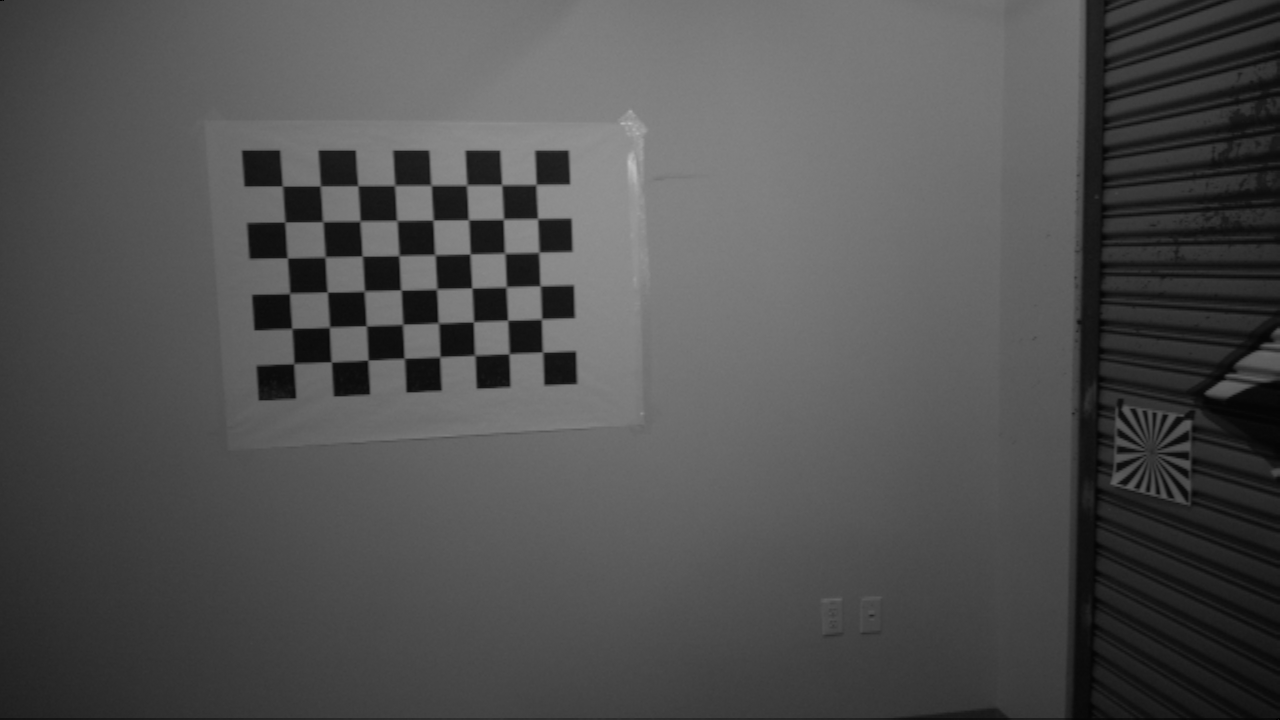
\includegraphics[width=1.0\textwidth]{img/calibration_grey}
		 \caption{}
	 \end{subfigure}
	 \begin{subfigure}{0.3\columnwidth} \centering
		 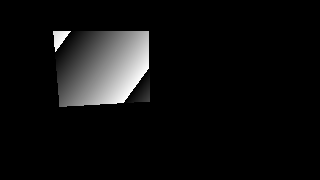
\includegraphics[width=1.0\textwidth]{img/calibration_model}
		 \caption{}
	 \end{subfigure}
	 	 \begin{subfigure}{0.3\columnwidth} \centering
		 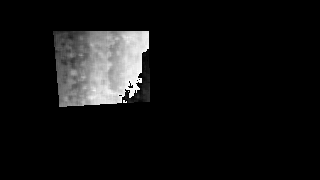
\includegraphics[width=1.0\textwidth]{img/calibration_data}
		 \caption{}
	 \end{subfigure}
	 \caption{Components collected in our calibration procedure. The greyscale (a)
	 image is used to compute a linear plane model (b) for depth. That model is
	 compared to the actual depth data (c) over a series of checkerboard poses.}
	 \label{fig:calibration}
 \end{figure}
 
 To train the distortion and noise model, we first calibrate the sensor with the
 use of a checkerboard calibration target. Images of the target are taken at
 multiple distances and angles from the camera (Fig. \ref{fig:calibration}). We
 fit an ideal plane to the target to determine what the true distance should be
 at each pixel. Then, we perform quadratic regression on the depth readings
 against the predicted readings from the plane to find the per-pixel distortion
 coefficients. The coefficients are stored in a database for later use.

The function $\sigma_{z_p}$ is computed in a similar way, by computing a
histogram of standard deviations of the depth readings, and then performing
quadratic regression on the result. A single function $\sigma_{z_p}$ is used for
the entire image, unlike the distortion model which is computed on a per-pixel
basis.

Finally, we preprocess all depth images from the device by inverting the
distortion model to get an estimate of the true depth at each point on the
image plane.

\subsection{The Signed Distance Function}
We model the world as a volumetric function $\Phi(x) : \mathbf{R}^3 \to
\mathbf{R}$, where, for every 3D point in the world, we have its distance to the
nearest surface of an object. Inside objects, the value of $\Phi$ is negative.
Outside objects, the value of $\Phi$ is positive, and on the surface, it is
zero.

 We will assume that $\Phi$ is static (\textit{i.e} it contains no moving
 objects aside from the sensor itself). We want to estimate the value of $\Phi$
 from the depth data and sensor poses over time.

Consider the geometry of the ideal depth sensor. Rays emenate from the sensor
origin to the scene. Call the origin of the ray $o$, and the endpoint of the ray
$x$. The direction of the ray is given by $r = \frac{o - x}{\|o - x\|}$.

The endpoint of each ray represents a point on the surface. So if the sensor is
perfect, we know that the signed distance function $\Phi(x) = 0$ at that point. 

But what else does the ray tell us? All the points in space along the ray from
the sensor origin up to the endpoint must be outside of any surface (or else the
ray would have been occluded by a a surface). Assuming objects have non-zero
thickness, some part of the space along the ray beyond the endpoint should be
inside an object. 

% That is:
% 
% \begin{equation}
% \Phi(x - ur) 
%      \begin{cases}
%      > 0 & \text{if } u > 0 \\
%      < 0 & \text{if } u < 0 \\
%      0 & \text{if } u = 0
%      \end{cases}
% \end{equation} 

Further, very near the surface of the object, the signed distance function can
be approximated by the distance along the ray to the endpoint of  the ray
(Figure \ref{fig:raycast_diagram}). This is because we know that there is at
least one point of the surface, namely the endpoint of the ray.  Near $x$, the
signed distance function is approximately the distance to $x$. So, whenever
$|u|$ is very small:

\begin{equation} 
\label{eq:pointwise_tsdf} 
	\Phi(x - ur) \approx u 
\end{equation}

Note that this approximation is better whenever the ray is approximately
perpendicular to the surface, and worst whenever the ray is parallel to the
surface. Because of this, some works \cite{Bylow2013} instead approximate
$\Phi$ by locally fitting a plane around $x$, and using the distance to that
plane as a local approximation, \emph{i.e}:

\begin{equation} 
\label{eq:planar_tsdf} 
	\Phi(x - ur) \approx -u~r \cdot n_x
\end{equation}

\noindent where $n_x$ is the local surface normal around $x$. In general, the
planar approximation (Eqn. \ref{eq:planar_tsdf}) is much better than the
pointwise approximation (Eqn. \ref{eq:pointwise_tsdf}), especially when surfaces
are nearly parallel to the sensor -- but computing surface normals is not
always computationally feasible. In our work, we have chosen to use
the simpler pointwise approximation.

\begin{figure}
   \begin{subfigure}{1.0\columnwidth}
     \centering
         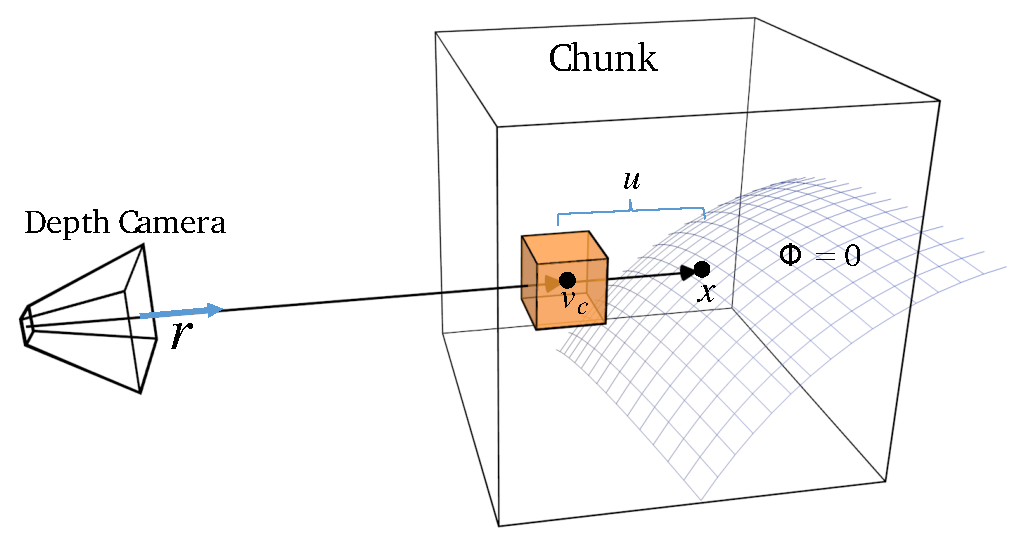
\includegraphics[width=1.0\textwidth]{img/Raycast}
      \caption{}
  \label{fig:raycast_diagram}
   \end{subfigure}
      \begin{subfigure}{1.0\columnwidth}
     \centering
         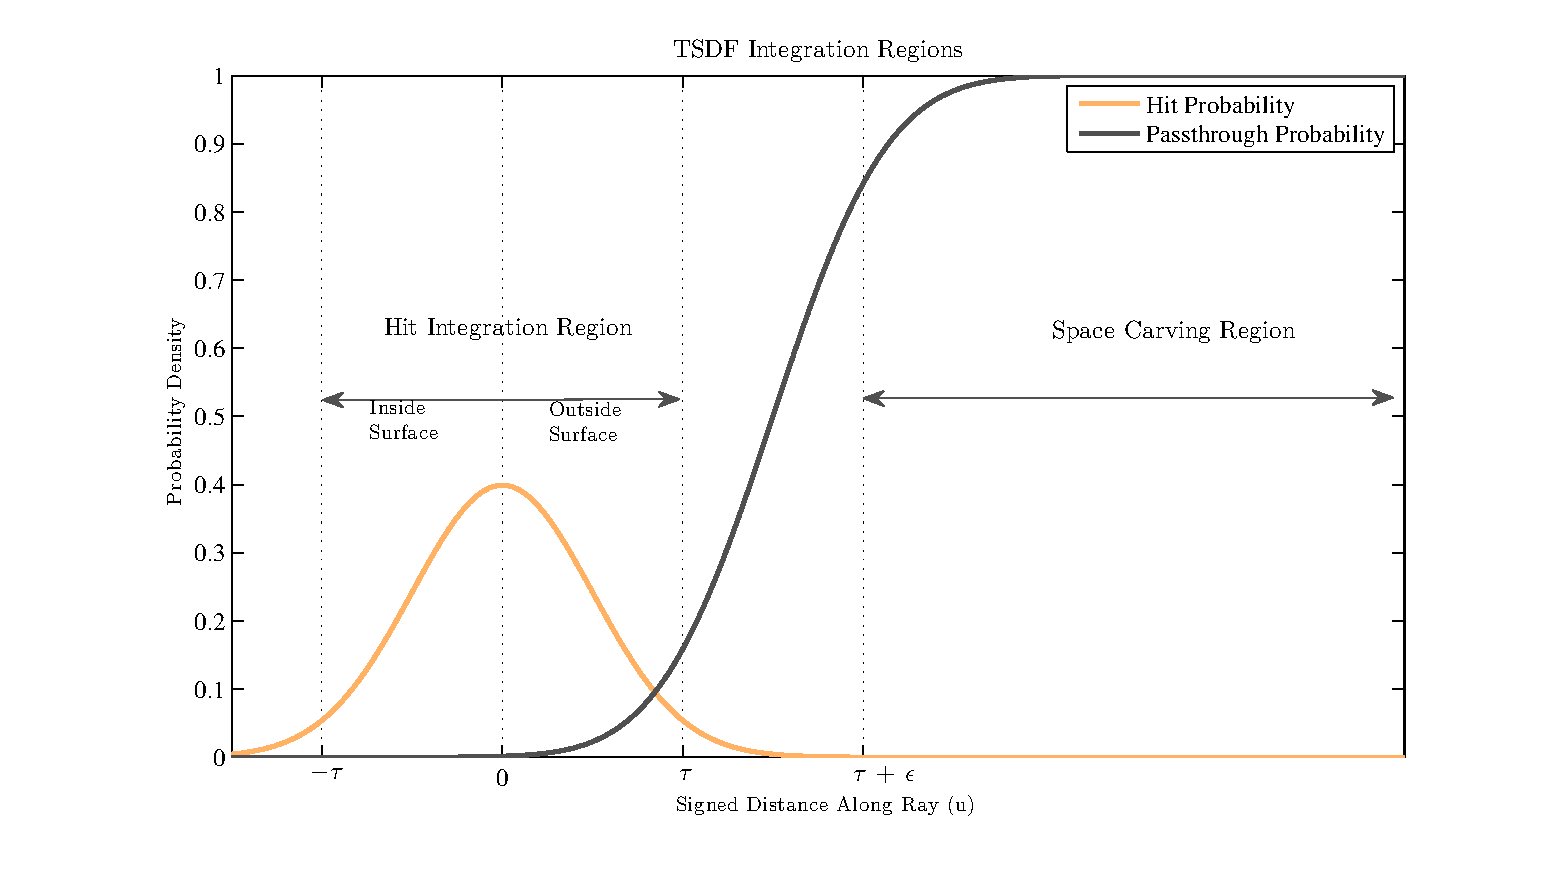
\includegraphics[ width=1.0\textwidth]{img/tsdf_integration.pdf}
         \caption{}
  \label{fig:integration_diagram}
   \end{subfigure}
   \caption{Figure (\ref{fig:raycast_diagram}) is a diagram of a ray hitting a
   surface from the camera, and a voxel that the ray passes through. The length of the ray from the point at
      which the ray intersects the voxel and the surface, $u$, is an
      approximation of the signed distance function $\Phi$, when $u$ is small.
      Figure (\ref{fig:integration_diagram} ) shows a hypothetical plot of the
      hit probability of a ray $P\left(z_p = \|x - u \cdot r\|\right) $, the pass probability $P\left(z_p
      < \|x - u \cdot r\|\right)$, vs. $u$. The hit integration region is inside $[-\tau,
      \tau]$, wheras regions closer to the camera than $\tau + \epsilon$ are in
      the space carving region (Section \ref{section:carving}). } 
\end{figure}


This observation leads us to the Truncated Signed Distance Function (TSDF)
\cite{Curless1996}. The TSDF is an approximation of the  Signed Distance
Function which stores distances to the surface within a small truncation
distance, $\tau$. That is:

\begin{equation} 
\Phi_{\tau}(x) \begin{cases}
	 = \Phi(x) & \text{if } |\Phi(x)| \leq \tau \\ 
	 \text{undefined} & \text{otherwise}
	 \end{cases}
\end{equation}

Following \cite{Curless1996}, to update the TSDF with a particular sensor
measurement, we integrate along the ray from $u = -\tau$ to $\tau$, and take the
weighted running average of distance field estimates over time, weighting by the
probability distribution of the sensor.

To do this, one can introduce a global weighting function $W : \mathbf{R}^3 \to
[0, 1]$ that represents the confidence in the estimate of the TSDF at every
point in space.

The process begins with 

\begin{align}
\Phi_{\tau}(x)& = \text{undefined} \;&\forall x  \\
%
 W(x)&= 0 \; &\forall x 
\end{align}

Then, for each ray and $u\in[-\tau, \tau]$:

\begin{subequations}
\begin{align}
\Phi_{\tau}(x - ur) \gets \frac{w_u \Phi_{\tau}(x - ur) + \alpha_u u}{w_u
+\alpha_u}
\\
%
w_u \gets w_u+ \alpha _u
\end{align}
\label{eqn:update}
\end{subequations}

\noindent Where  $w_u = W(x - ur)$, and $\alpha_u  = \alpha(u) : [-\tau,\tau]\to
\mathbf{R} $ is a weighting function which normalizes to 1 over the truncation
distance . Ideally, the weighting function should be determined by the
probability distribution of the sensor, and should represent the probability
that $\Phi(x - ur) = 0$. It is possible \cite{Nguyen2012} to directly compute
the weight from the probability distribution of the sensor, and hence compute
the actual \emph{expected} signed distance function.In favor of better
performance, linear, exponential, and constant approximations of $\alpha_u$ can be used \cite{Curless1996, Newcombe,
Whelan2013, Bylow2013}.

In our work, we simply use a constant approximation $\alpha(u) = \frac{1}{2
\tau}$, and use the probability distribution of the sensor instead to 
dynamically select the value of $\tau$, as in \cite{Nguyen2012} (Fig.
\ref{fig:integration_diagram}). This results in poorer surface reconstruction
quality in areas of high noise than methods which more closely approximate the
hit probability of the sensor.

\subsection{Colorization}
To create colored surface reconstructions, we use a method following Bylow et.
al \cite{Bylow2013}, also used in \textit{Kintinuous} \cite{Whelan2013}, which
directly stores color information as volumetric data. Alongside the
truncated signed distance function, we store a volumetric color function
$C_\tau : \mathbf{R}^3 \to \mathbf{R}^3$, and a color weighting function $W_c :
\mathbf{R}^3 \to \mathbf{R}$.

Color is updated in exactly the same manner as the TSDF. We assume that each
depth ray also corresponds to a color in the RGB space. We integrate along the
ray from $u \in [-\tau, \tau]$, and update the color:

\begin{align}
C(x - ur) \gets \frac{w_c C(x - ur) + \alpha_c \mathbf{c}}{w_c}
+\alpha_c
\\
%
w_c \gets w_c + \alpha_c
\end{align}

\noindent where $\mathbf{c} \in \mathbf{R}^3$ is the color of the ray in RGB
space, $\alpha_c$ is a color weighting function, and $w_c = W_c(x -
ur)$.

In both \cite{Bylow2013} and \cite{Whelan2013}, the color weighting function is
proportional to the dot product of the ray's direction and an estimate of the
surface normal. But since surface normal estimation is computationally
expensive, we instead use the same weight for both distance and color.

We must also deal with the fact that color images and depth data may be
asynchronous. In our case, depth data is often delayed behind color data by as
much as 30 milliseconds. So, for each depth scan, we project the endpoints of
the rays onto the nearest color image in time to the depth image, disregarding
occlusion, and use bilinear interpolation on the color image to determine the
color of each ray.

\subsection{Dynamic Truncation Distance}
Following the approach of Nguyen et. al \cite{Nguyen2012}, we use a dynamic
trunction distance based on the noise model of the sensor rather than a fixed
truncation distance. In this way, we have a trunction function:

\begin{equation} \tau(z_u) = \beta\sigma_{z_u} \end{equation}

Where $\sigma_{z_u}$ is the standard deviation of the noise for a depth reading
of $z_u$, and $\beta$ is a scaling parameter which represents the number of
standard deviations of the noise we want to integrate over.

Using the dynamic truncation distance has the effect that further away from the
sensor, where depth measurements are less certain and sparser, depth
measurements are smoothed over a larger area of the distance field; while nearer
to the sensor, where depth measurments are more certain and closer together, the
truncation distance is smaller.

\subsection{Space Carving}
\label{section:carving}
When depth data is highly noisy and sparse, the relative importance of negative
data (that is, information about what parts of the space do not contain an
obstacle) increases over positive data \cite{Klingensmith2014}. This is because
rays passing through empty space constrain possible values of the signed
distance field to be positive at all points along the ray, wheras rays hitting
objects only inform us about the presence of a surface very near the endpoint of
the ray. In this way, rays can be viewed as \textit{constraints} on possible
values of the distance field. 

For this reason, we augment our TSDF algorithm with a \textit{space carving}
constraint. Along each ray from $u \in [0, \tau - \epsilon]$ (where $\epsilon$
is a small value that prevents carving of space near surfaces) called the space
carving region (Fig. \ref{fig:integration_diagram}), we set:

\begin{align}
\Phi_{\tau}(x - ur) \gets \text{undefined}
\\
%
w_u \gets 0
\end{align}

\noindent  The effect is that, as rays pass through previously integrated
regions of the TSDF, they clear away inconsistent data. Similarly, colors are
cleared away whenever rays pass through previously colored space.

Space carving gives us two advantages: first, it dramatically improves the
surface reconstruction in areas of very high noise (especially around the edges
of objects), and second, it removes some inconsistencies caused by moving
objects and localization errors. If space carving is not used, moving objects
appear in the TSDF as permanent blurs, and localization errors result in
multiple overlapping isosurfaces appearing. With space carving, old inconsistent
data is removed and only the latest data is used.

\subsection{Implementation: Chunked TSDF}
We use a discrete approximation of the TSDF which divides the world into
a uniform 3D grid of voxels. Each voxel contains an estimate of the signed
distance function and an associated weight. In our implementation, these are
packed into a single 32-bit integer. The first 16 bits are a fixed-point
signed distance value, and the last 16 bits  are an unsigned integer weighting
value. Color is similarly stored as a 32 bit integer, with 8 bits per color
channel, and an 8 bit weight. A similar method is used in \cite{Newcombe,
Whelan2013, Bylow2013} to store the TSDF.

Unfortunately, a flat volumetric representation of the world using voxels is
incredibly memory intensive. The amount of memory storage required grows as
$\mathcal{O}(N^3)$, where $N$ is the number of voxels per side of the 3D voxel
array.

For example, at a resolution of $3\text{cm}$,  a $30\text{m}$ TSDF cube with
color would occupy 8 Gigabytes of memory. Worse, most of that memory would be
uselessly storing unseen free space. Further, if we plan on exploring larger and larger
distances using the mobile sensor, the size of the TSDF array must grow if we
don't plan on allocating enough memory for the entire space to be explored.

For a large-scale real-time suface reconstruction application, a less
memory-intensive and more dynamic approach is needed. Confronted with this
problem, other approaches have either used  octrees \cite{Wurm2010}, or have
prematurely extracted isosurfaces from a moving TSDF volume to save memory
\cite{Whelan2013}.

Neither of these approaches is desirable for our application. Octrees, while
maximally memory efficient, have significant drawbacks when it comes to
accessing and iterating over the volumetric data.

An octree compresses volumetric data by dividing the space recursively into
octants. The leaves of the tree contain the underlying volumetric data. Octants
which contain no leaves do not contain any allocated volumetric data. This
allows the octree to be incredibly memory efficient if the underlying
volumetric data is sparse.

However, consider that every time an octree is \emph{queried}, one incurs a
logarithmic $\mathcal{O}(K)$ cost, where $K$ is the depth of the Octree. In
contrast, queries in a flat array are $\mathcal{O}(1)$. This might not seem so
bad, until one considers the overhead of traversing an octree. If implemented na\"{\i}vely, an
octree will be implemented by storing pointers to child octants in each parent
octant, and worse, the octants may be dynamically allocated on the heap. Each
traversal through the tree requires $\mathcal{O}(K)$ heap pointer
dereferences in the worst case. Even worse, adjacent voxels may not be adjacent
in memory, resulting in very poor caching performance.

Instead of using an Octree, or a fixed 3D array (as in \cite{Newcombe,
Whelan2013}), we use a hybrid data structure which maintains some of the
advantages of both. 

\begin{figure}
  \centering
  	\begin{subfigure}{0.48\columnwidth} \centering
    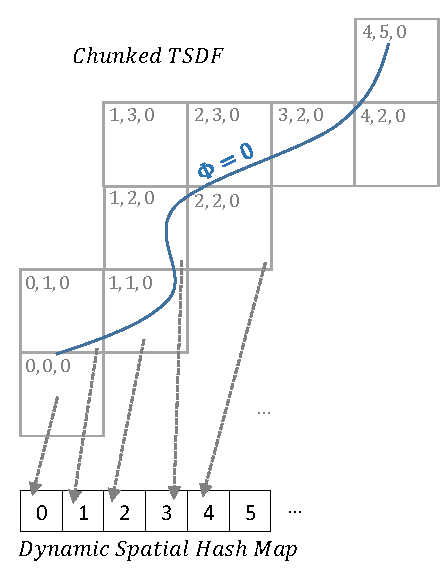
\includegraphics[width=1.0\textwidth]{img/chunks.pdf}
      \caption{}
  	\label{fig:chunks} 
  \end{subfigure} 
  \begin{subfigure}{0.48\columnwidth} \centering
      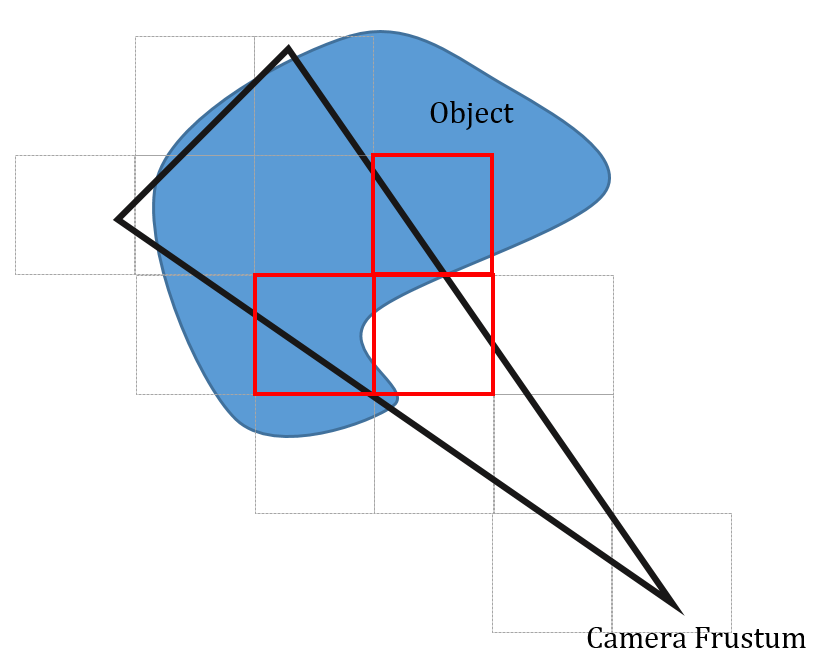
\includegraphics[width=1.0\textwidth]{img/frustum_cull}
      \caption{}
 	 \label{fig:frustum_cull}
  \end{subfigure}
  \caption{In Fig. \ref{fig:chunks}, chunks of voxels (grey) are allocated near
  the surface (blue) of the scene. Chunks are spatially hashed \cite{SpatialHashing} into a
      dynamic hash map. Lookups into the hash map are constant time. Within each
      chunk, voxels are allocated in a 3D array. Fig.
      \ref{fig:frustum_cull} shows all the TSDF chunks which intersect the depth
      camera frustum  and are within $\tau$ of a hit as green cubes. Only these
      chunks are updated when new data is received. The scene shown is a
      reconstruction of the Freiburg office \cite{FREIBURG} dataset at a
      resolution of 3cm}
\end{figure} 

We divide the world into a two-level tree. In the first level we have
\emph{chunks} of voxels (Figure \ref{fig:chunks}). Each chunk consists of a
fixed grid of $N_c^3$ voxels, which are stored in a flat 3D array. Chunks are
allocated dynamically from a growing pool of heap memory as data is added, and
are indexed in a spatial 3D hash map \cite{SpatialHashing} by their spatial
coordinates. Following Teschner \emph{et. al} \cite{SpatialHashing}, we use the
hashing function:

\begin{equation}
\textbf{hash}(x, y, z) = p_1 x\oplus p_2 y \oplus p_3 z
~\text{mod}~n
\end{equation}

\noindent where $x, y, z$ are the 3D integer coordinates of the chunk, $p_1,
p_2, p_3$ are arbitrary, large primes, $\oplus$ is the xor operator, and $n$ is
the maximum size of the hash map.

Since chunks are a fixed size, querying data from the chunked TSDF involves
rounding (or bit-shifing, if $N_c$ is a power of two) a world coordinate to a
chunk and voxel coordinate, and then doing a hash-map lookup followed by a 3D
array lookup. Hence, querying is $\mathcal{O}(1)$. Further, since voxels within
chunks are stored adjacent to one another in memory, cache performance is
improved while iterating.

By carefully selecting the size of chunks so that they coresponding to $\tau$,
we only allocate volumetric data near isosurfaces of objects, and do not waste
memory on empty space.

\subsection{Depth Scan Integration}
\label{section:scan_integration}
To perform the process described in Eqn. \ref{eqn:update}, it is necessary
to consider each ray in each depth scan and upate each voxel
along the ray according to its distance to an observed isosurface.

The most straightfoward way of doing this is to simply iterate over each ray,
and then use a fast rasterization algorithm \cite{RayTracing} to determine which
voxels intersect with the ray. We will call this the \textit{Raycasting}
approach. However, this approach is extremely computationally expensive, having
a performance bound by $\mathcal{O}(N_{\text{ray}} \times
l_{\text{ray}})$, where $(N_{\text{ray}}$ is the number of rays ina 
scan, and $l_{\text{ray}}$  is  proportional to the length of a ray
being integrated. If we use a fixed-size truncation distance and do not perform 
space carving, $l_{\text{ray}} = \tau$. However, with space-carving,
the length of a ray being integrated is potentially unbounded.

A useful approximation of raycasting is \textit{projection mapping}. Used in
\cite{Nguyen2012, Bylow2013, Klingensmith2014}, projection mapping works by
projecting points in the voxel grid onto the depth image and comparing the depth value
there with the geometric distance from the center of the voxel to the camera
plane, and using that to approximate the distance along the ray from the camera
to the voxel. This is analagous to \textit{shadow mapping} \cite{Shadowmapping}
from computer graphics, where raycast shadows are approximated by projecting
onto a depth map from the perspective of the light source, except in our case, 
``shadows'' are regions occluded from the depth sensor.  

\begin{figure}
  \centering
    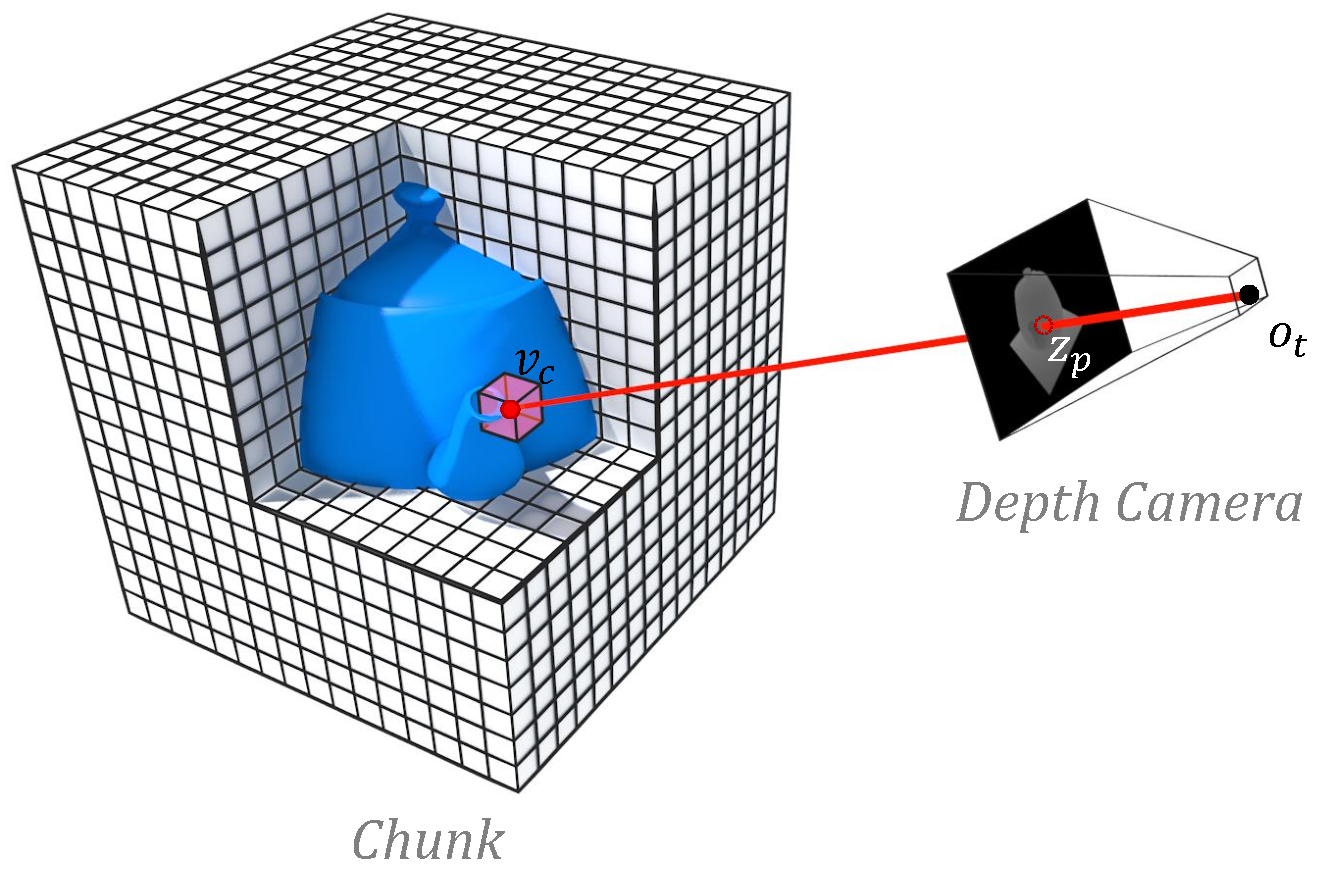
\includegraphics[width=0.95\columnwidth]{img/projection_mapping}
      \caption{A cutaway of a chunk containing an object is shown. In projection
      mapping,  a particular voxel with center $v_c$ is projected onto the depth
      camera at time $t$. The depth image is binlinearly interpolated to get
      $z_p$, a depth reading at the projected point. This is compared to the length of the vector
      from the voxel center $v_c$ to the camera origin $o_t$ to approximate the
      distance to the surface. This is repeated for every voxel in the chunk.}
  \label{fig:projection_mapping} 
\end{figure} 


For each voxel in a chunk that is to be updated, we take its center $v_c$, and
project it onto the depth image using the camera intrinsics and a pinhole camera
model. We then use bilinear interpolation of the depth values to find an
expected depth reading $z_p$. Call origin of the sensor  $o_t$,   then the 
distance from the sensor to the voxel is $\|o_t - v_c\|$ (Fig. \ref{fig:projection_mapping}).

Now, if the isosurface passes directly through the center of the voxel,
then we should expect that $z_p = \|o_t - v_c\|$, and, in particular, the
distance along the ray to the isosurface is approximated by $u' = z_p - \|o_t -
v_c\|$ to update the voxel according to Eqn. \ref{eqn:update}.

Projection mapping has performance bounded by $\mathcal{O}(N_v)$, where $N_v$ is
the number of voxels affected by a depth scan. This value is nearly constant
over time, and depending on the resolution of the TSDF, may be significantly
less than the number of points. When using space carving (Section
\ref{section:carving}), raycasting has an additional performance hit bounded by
the length of the rays, wheras projection mapping does not suffer from this
performance hit.

However, projection mapping suffers from resolution-dependant aliasing errors,
because the value of $u'$ taken from projection mapping may differ from the true
depth of the ray by up to the length of the diagonal of the voxel. Nuanced
surface information from many adjacent rays passing through a single voxel is
lost in the projection mapping case. This can be mitigated somewhat by
\textit{oversampling} each voxel (that is, considering many sampled points
inside each voxel) and taking the average projected depth over all the samples
-- but the speed of the approach decreases linearly with the number of 
additional samples taken. 

\subsection{Frustum Culling and Garbage Collection}
To determine which chunks should be updated by a depth scan, and which chunks
should be drawn, we use frustum culling. We first construct a conservative
geometric convex approximation of the space visible to the depth camera by
creating a camera frustum (\textit{i.e.} a truncated pyramid) with a far plane
at the maximum depth reading of the camera, and the near plane at the minimum
depth of the camera. 

We then take the axis-aligned bounding box of the camera frustum in the global
frame, and check each chunk inside the axis-aligned bounding box for 
intersection with the camera. Only those which intersect the frustum are
updated. If chunks that would intersect the frustum haven't been allocated yet,
they are allocated before a depth scan is inserted.

Since the frustum is a conservative approximation of the space that could be
updated by a depth scan, some of the chunks that are visible to the frustum will
have no depth data associated with them. For this reason, we also store a flag
inside each chunk indicating whether or not that chunk ever contained the
endpoint of a ray from the depth camera (Figure \ref{fig:frustum_cull}).

Those chunks which do not get updated during a depth scan are garbage collected
(deleted from the hash map), reducing memory overhead.

\subsection{Rendering}
In the original \textit{Kinect Fusion} work \cite{Newcombe}, rendering was
accomplished by raytracing on the GPU. Raytracing has the advantage of being a
pixel-perfect representation of the surface, and performance scales only with
the resolution of the rendering rather than with the size of the space. 

However, real-time raytracting requires intensive GPU computation that we simply
do not have on the mobile device. For that reason, it is necessary to develop a
real-time rendering solution that is amenable to the limited graphics
capabilities of mobile devices.

We have decided to use a technique of incremental Marching Cubes
\cite{Lorensen1987} to render the TSDF. For each chunk, we store a triangle
mesh. Triangle meshes are generated at the isosurface $\Phi_{\tau}(x) = 0$
whenever the chunk has been updated by a depth scan since the last time the
chunk was rendered. As in \cite{Bylow2013, Whelan2013},  colors are computed for
each vertex by trilinear interpolation of the color map. At the borders of chunks, vertices are
duplicated to reduce co-dependence between the chunks, at the expense of
causing slight seams between chunk meshes.

Only those meshes which are visible to the virtual camera frustum are rendered.
Meshes that are very far away from the camera are rendered as a colored bounding
box.

Using incremental Marching Cubes allows us to render the scene using only simple
fixed function pipeline calls on the device's graphics hardware. This is
important for many mobile devices where the fixed function pipeline is all that
is available. It also allows us to produce surface meshes asynchronously from
depth image updates and rendering, as (except for the edges of  each chunk) the
surface meshes are indepent of each other.

\subsection{Pose Estimation}
We will assume we  have \textit{a priori} black-box pose estimation of
the sensor from a seperate tracking system. Specifically, in our experiments,
pose data is estimated from an onboard visual-intertial odometry system that
fuses data from a wide-angle camera, an intertial measurement unit, and a
gyroscope at 60 Hz using 2D feature tracking and an Extended Kalman Filter. A
more detailed discussion of this system can be found in \cite{VINS}. 

Unlike \textit{Kinect Fusion} \cite{Newcombe} and \textit{Kintinuous}
\cite{Whelan2013}, our approach makes no attempt to estimate the pose of the
sensor directly from depth data. Instead, we use depth data only for surface
reconstruction. Unfortunately, decoupling the pose estimation and surface
reconstruction results in failure to correct for drift in the pose estimation
using depth data, and can result in mis-alignment of depth scans (Fig.
\ref{fig:gameroom_vio}).

% Section removed to save space
% \subsubsection{Pose Interpolation}
% We will assume that pose estimation, depth sensing, and color sensing are
% asynchronously executed, so we may not have all three measurements at a given
% time. To deal with asynchronous sensing and pose estimation, we linearly
% interpolate poses over time to determine the pose of a given sensor at any given time.
% 
% Call the global pose estimate of the sensor at time $t$,  ${H_{s}}^t$.
% Additionally, assume we have apriori extrinsic pose estimates for the color
% sensor ${E_{c}}$ and the depth sensor ${E_{d}}$. We are given a discrete
% trajectory of pose estimates from the visual-inertial odometry system:
% 
% $$ {H_{s}}^{t_1}, {H_{s}}^{t_2}, \ldots, {H_{s}}^{t_T} $$
% 
% Suppose at time $t'$, we get a color image. Assume that $t'$ is not represented
% in the list of sensor body poses. Then, either $t' < t_1$,  $t' > t_T$, or
% $t_a < t < t_b'$ for some $a, b \in [1, T]$. In the first case ($t' < t_1$), we
% disregard the color image. In the second case ($t' > t_T$), we wait until more data is
% acquired. In the third case, we would interpolate the pose of the color camera
% as:
% 
% $$ {H_{c}}^{t'} \approx E_c \cdot \textbf{Interp}\left(H_{s}^{t_a}, H_{s}^{t_b},
% \frac{t' - t_a}{t_b - t_a}\right) $$
% 
% Where $\textbf{Interp}$ is a function that  interpolates between two
% poses by linearly interpolating translation while spherically interpolating
% rotation, using $\frac{t' - t_a}{t_b - t_a} \in [0, 1]$ as an interpolation
% parameter. 

% Section removed to save space
% \subsection{User Interface}
% We developed a simple and intuitive prototype interface to test our approach on
% the device. Users were presented with options for controlling the resolution of
% the reconstruction, and were able to control when the system was active and
% inactive, allowing them to pause when moving objects obscured objects they were
% trying to model.
% 
% We present the user with camera controls as well. A virtual first person
% camera mimics the intrinsics of the depth camera. A third-person camera allows
% the user to rotate the virtual camera around their current position and get a
% better look at the quality of the reconstruction; and an orthographic overhead
% camera functions as a global map of where the user has been (Figure
% \ref{fig:map_device}).
% 
% At any time, the user can save the volumetric representation of the TSDF, or a
% surface mesh generated by marching cubes to disk.

\section{Experiments and Results}
\begin{figure}
  \centering
    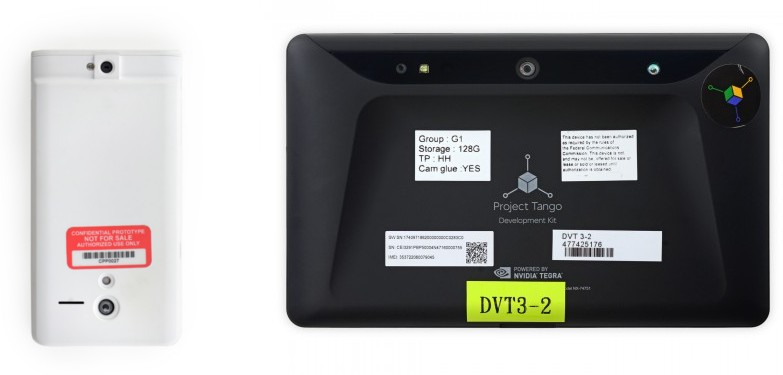
\includegraphics[width=1.0\columnwidth]{img/devices}
      \caption{The \textit{Tango}\cite{Tango} ``peanut'' phone (left), and
      ``yellowstone" tablet (right).}
  \label{fig:devices}
\end{figure}

\subsection{Hardware}
We implemented our approach on two devices: a \textit{Tango}
``yellowstone" tablet device, and a \textit{Tango} ``peanut'' mobile phone
device (Figure \ref{fig:devices}). The phone device has 2GB of RAM, a quadcore
CPU, a six-axis gyroscope and accelerometer, a wide-angle $120^\circ$ field of
view tracking camera which refreshes at 60Hz, a projective depth sensor which
refreshes at 6Hz, and a 4 megapixel color sensor which refreshes at 30Hz. The
tablet device has 4GB of ram, a quadcore CPU, an Nvidia Tegra K1 graphics card,
an identical tracking camera to the phone device, a projective depth sensor
which refreshes at 3Hz, and a 4 megapixel color sensor which refreshes at 30Hz.
Devices were depth calibrated \ref{subsection:calibration} prior to testing. 

\subsection{Large Scale Online Mapping}
 \begin{figure} \centering
	 \begin{subfigure} {0.6\columnwidth} \centering
		 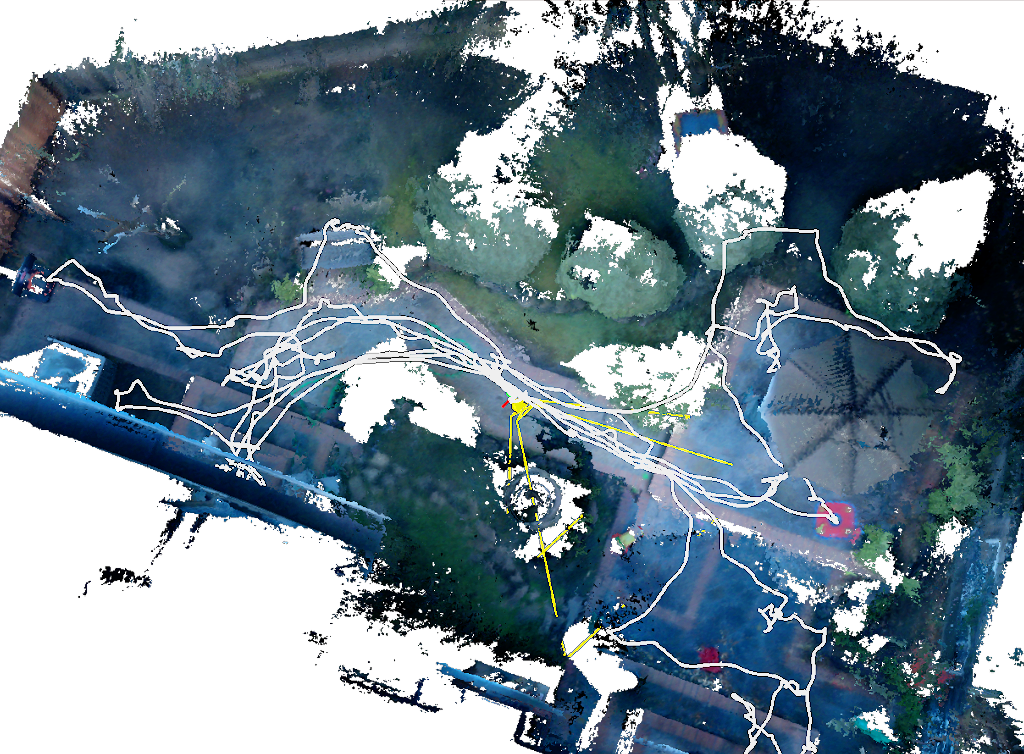
\includegraphics[width=1.0\textwidth]{img/colorbalance3}
		 \caption{}
		 \label{fig:overhead_night}
	 \end{subfigure}
	 \begin{subfigure}{0.44\columnwidth} \centering
		 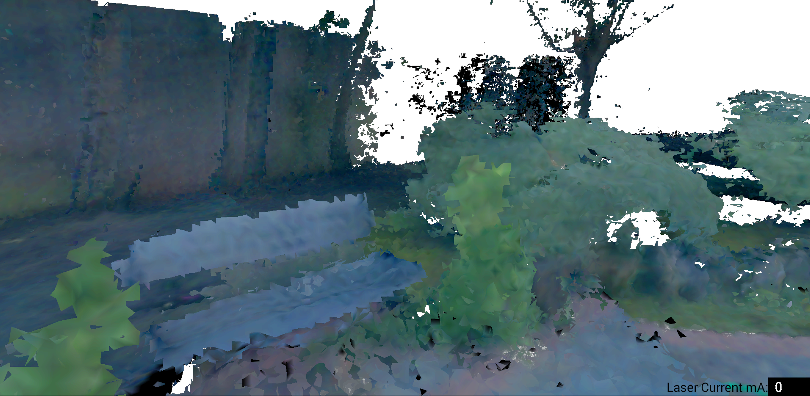
\includegraphics[width=1.0\textwidth]{img/colorbalance2}
		 \caption{}
		 \label{fig:night2}
	 \end{subfigure}
	 	 \begin{subfigure}{0.44\columnwidth} \centering
		 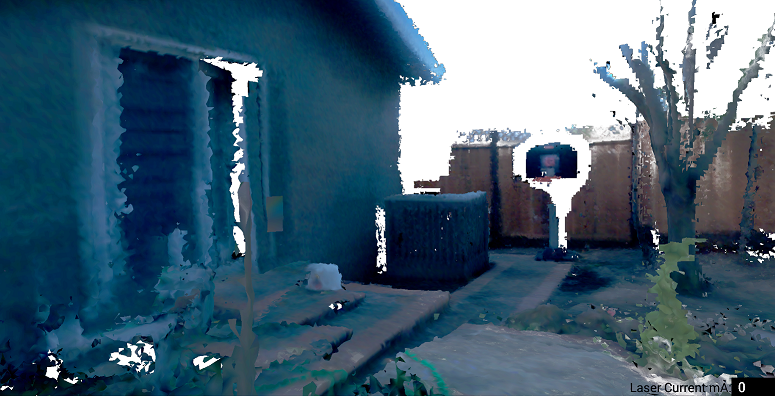
\includegraphics[width=1.0\textwidth]{img/colorbalance1} 
		 \caption{}
		 \label{fig:night3}
	 \end{subfigure} 
	 \caption{An outdoor scene captured at night with the yellowstone device at a
	 resolution of 3 cm. Figure \ref{fig:overhead_night} shows an overhead view of
	 the scene. The yellow pyramid represents the depth camera frustum. The white
	 lines are the aggregate trajectory of the device. Figures \ref{fig:night2}
	 and \ref{fig:night3} show closeups of the scene taken live from the device.
	 The scene was captured using projection mapping (Sec.
	 \ref{section:scan_integration}), without space
	 carving (Sec. \ref{section:carving})}
	 \label{fig:outside}
 \end{figure} 

Using our algorithm, we are able to create and display large scale maps at a
resolution as small as 3cm in real-time using only visual-intertial odometry for pose
estimation. Figure \ref{fig:map_device} shows a map of an office building floor
being reconstructed in real-time using the phone device. This scenario is also
shown in an attached video \cite{TangoVideo}. Using the tablet device, we have
reconstructed (nightime) outdoor scenes in real-time (Figure \ref{fig:outside}).

In the course of online mapping, the user has immediate feedback on model
completness, and can pause mapping for live inspection. The system continues
localizing the device using visual-intertial odometry even when the mapping is
paused. After mapping is complete, the user can save the map to disk.
 
\subsection{Comparing Depth Scan Integration Algorithms} 
  \begin{figure} \centering
	 \begin{subfigure} {0.4\columnwidth} \centering
		 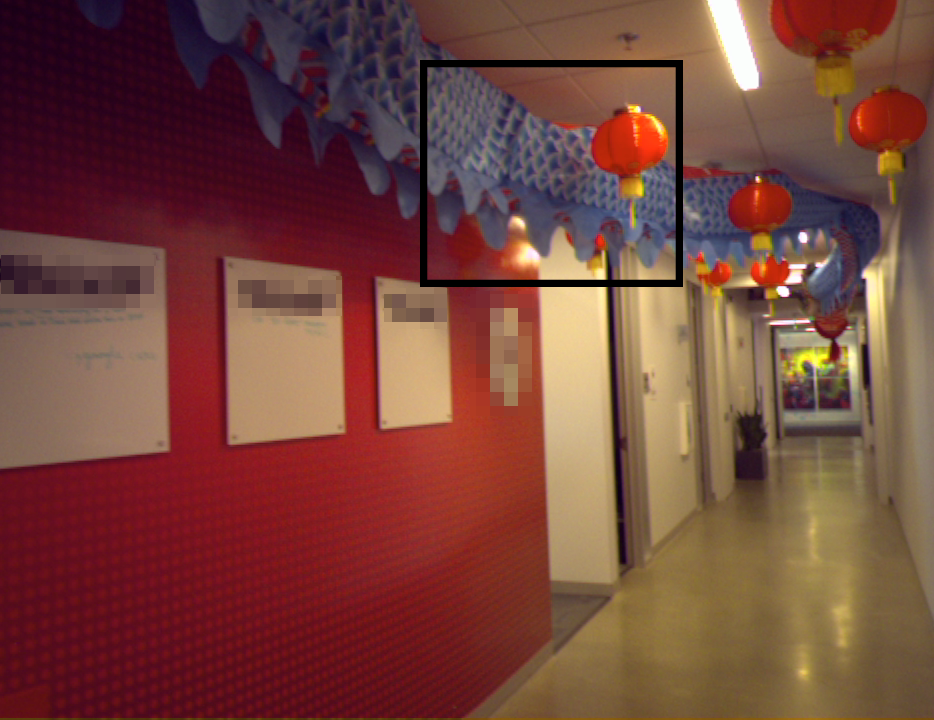
\includegraphics[width=1.0\textwidth]{img/dragon_color.png}  
		 \caption{}
		 \label{fig:dragon_color}
	 \end{subfigure}
	 \begin{subfigure}{0.4\columnwidth} \centering
		 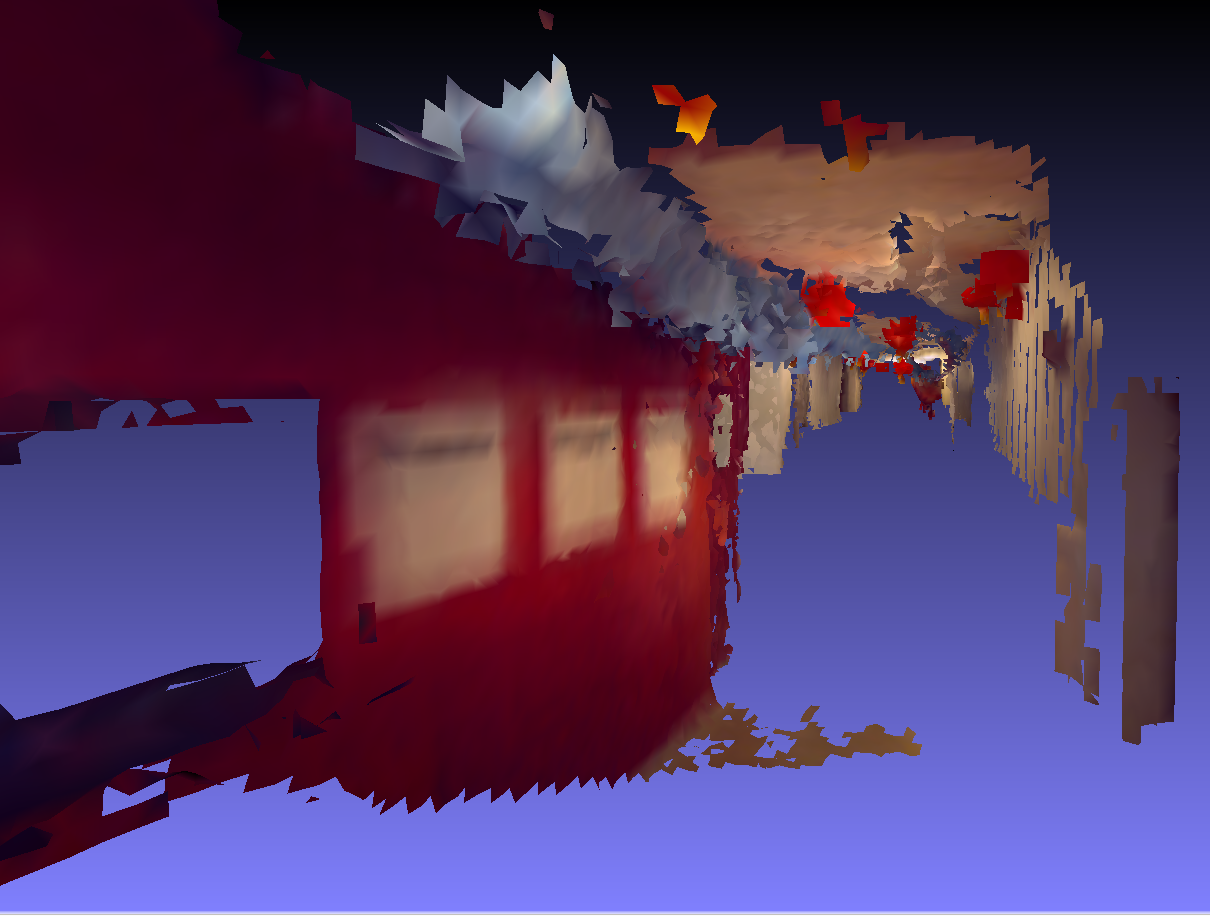
\includegraphics[width=1.0\textwidth]{img/dragon_projection_nocarve.png}
		 \caption{}
		 \label{fig:dragon_projection_nocarve}
	 \end{subfigure}
	 \begin{subfigure}{0.4\columnwidth} \centering
		 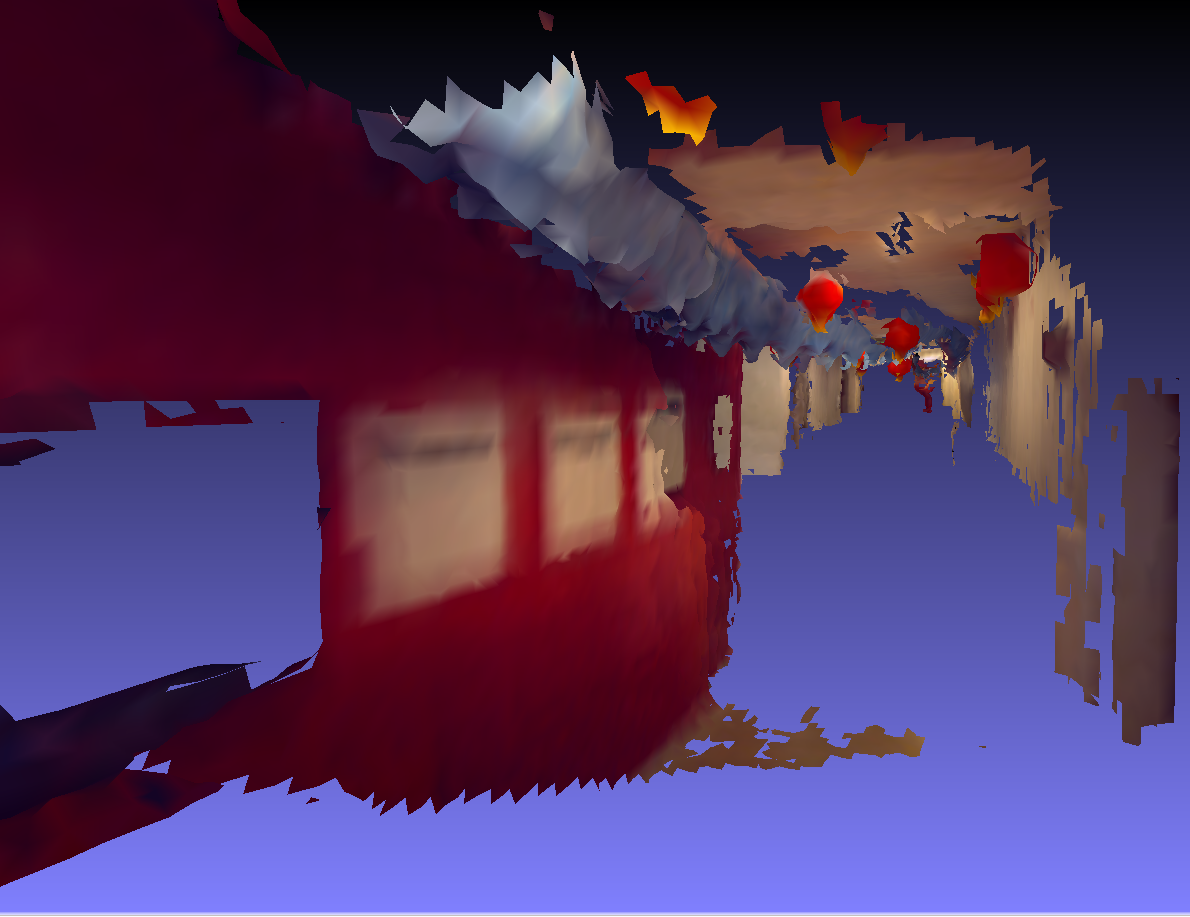
\includegraphics[width=1.0\textwidth]{img/dragon_projection_carve.png} 
		 \caption{}
		 \label{fig:dragon_projection_carve} 
	 \end{subfigure} 
	 \begin{subfigure}{0.4\columnwidth} \centering  
		 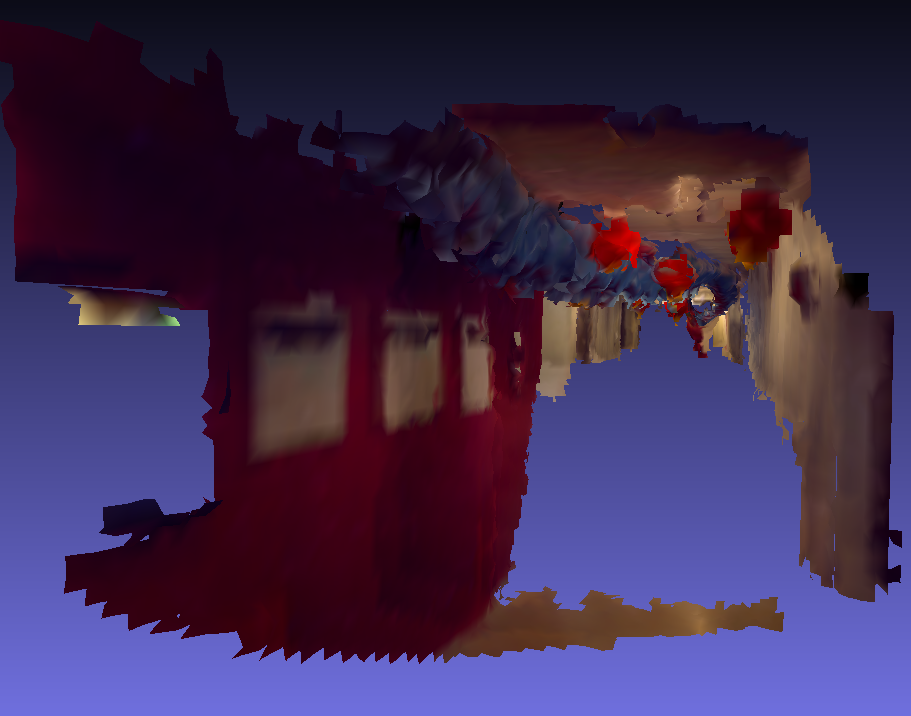
\includegraphics[width=1.0\textwidth]{img/dragon_raycast.png} 
		 \caption{}
		 \label{fig:dragon_raycast}
	 \end{subfigure} 
	 	 \begin{subfigure}{0.7\columnwidth} \centering  
		 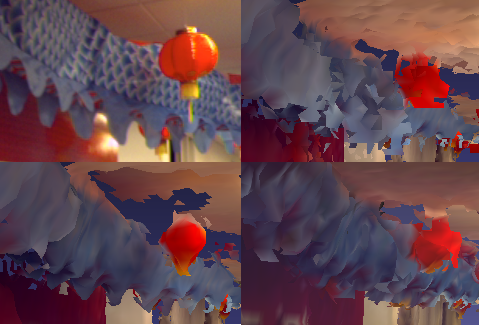
\includegraphics[width=1.0\textwidth]{img/dragon_closeup.png} 
		 \caption{}
		 \label{fig:dragon_closeup}
	 \end{subfigure} 
	 \caption{Different depth scan integration techniques are compared. Fig.
	 \ref{fig:dragon_color} shows the color image for reference. Fig.
	 \ref{fig:dragon_projection_nocarve} shows voxel projection without space
	 carving. Fig. \ref{fig:dragon_projection_carve} shows voxel projection with
	 space carving, and Fig. \ref{fig:raycast_diagram} shows raycasting without
	 space carving. Fig. \ref{fig:dragon_closeup} is a closeup of a lantern
	 in the scene; counter-clockwise from the top left: color image, projection
	 mapping without space carving, projection mapping with space carving, and raycasting
	 without space carving. During the scan, the user was looking mostly toward the
	 ceiling, at the colorful dragon.}
	 \label{fig:dragon}
 \end{figure}   
 
 
 \begin{figure}
  \centering
 \begin{subfigure}{0.75\columnwidth} \centering
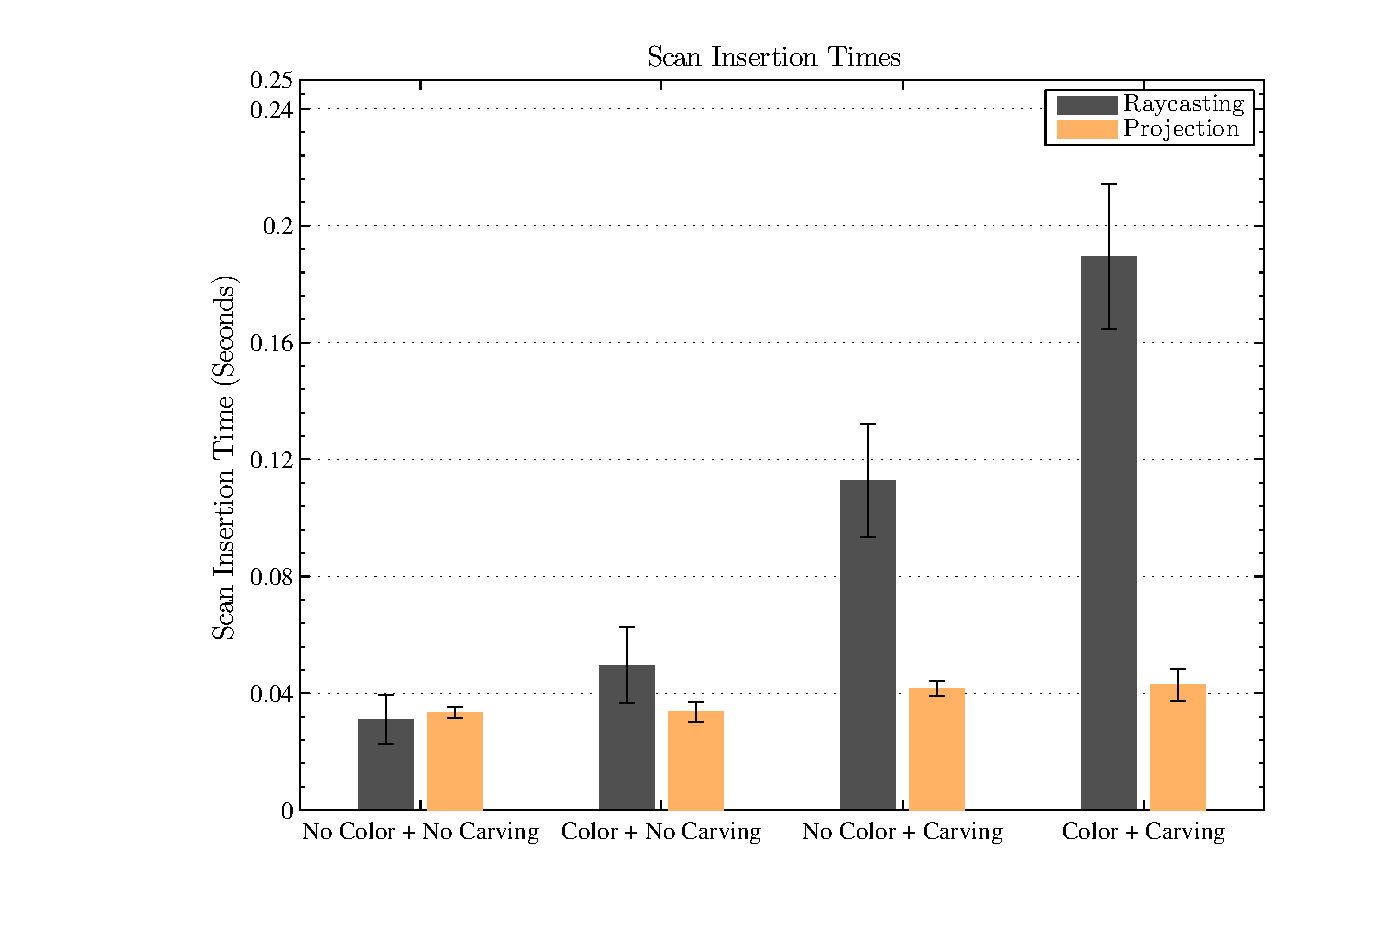
\includegraphics[width=1.0\textwidth]{img/timing_data.pdf}
		 \caption{}
		 \label{fig:timing}
	 \end{subfigure} 
 \begin{subfigure}{0.75\columnwidth} \centering
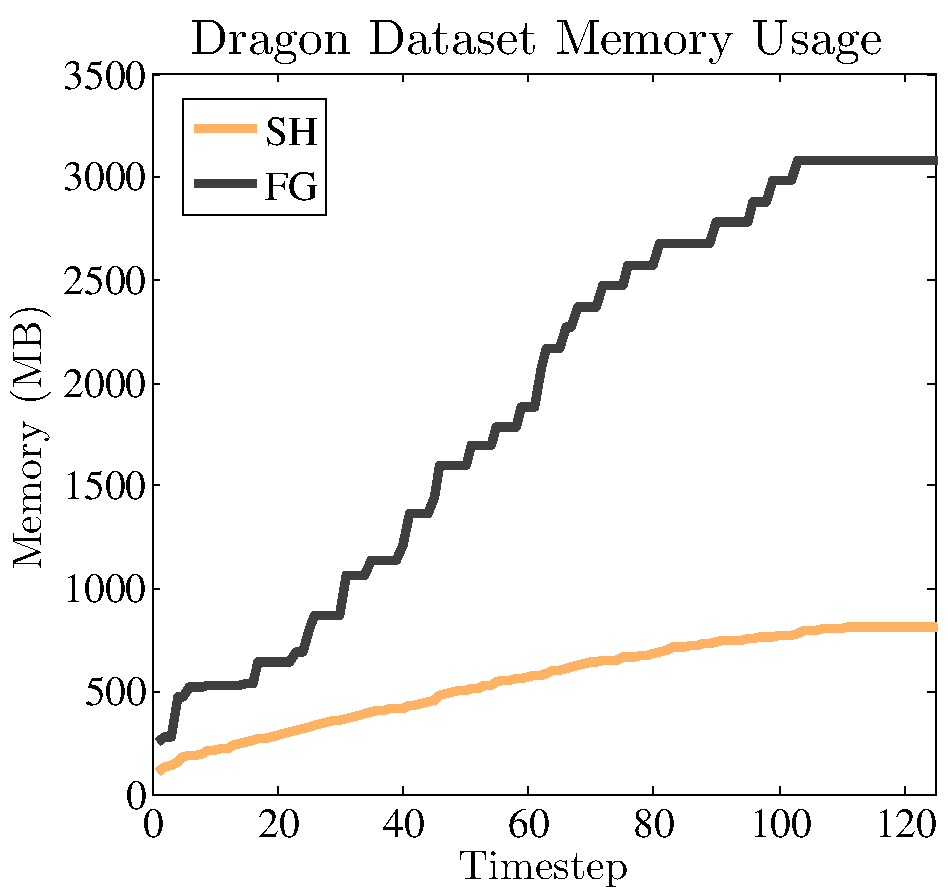
\includegraphics[width=1.0\textwidth]{img/memoryusage.pdf}
		 \caption{} 
		 \label{fig:memory_data}
	 \end{subfigure}  
	  \begin{subfigure}{0.75\columnwidth} \centering
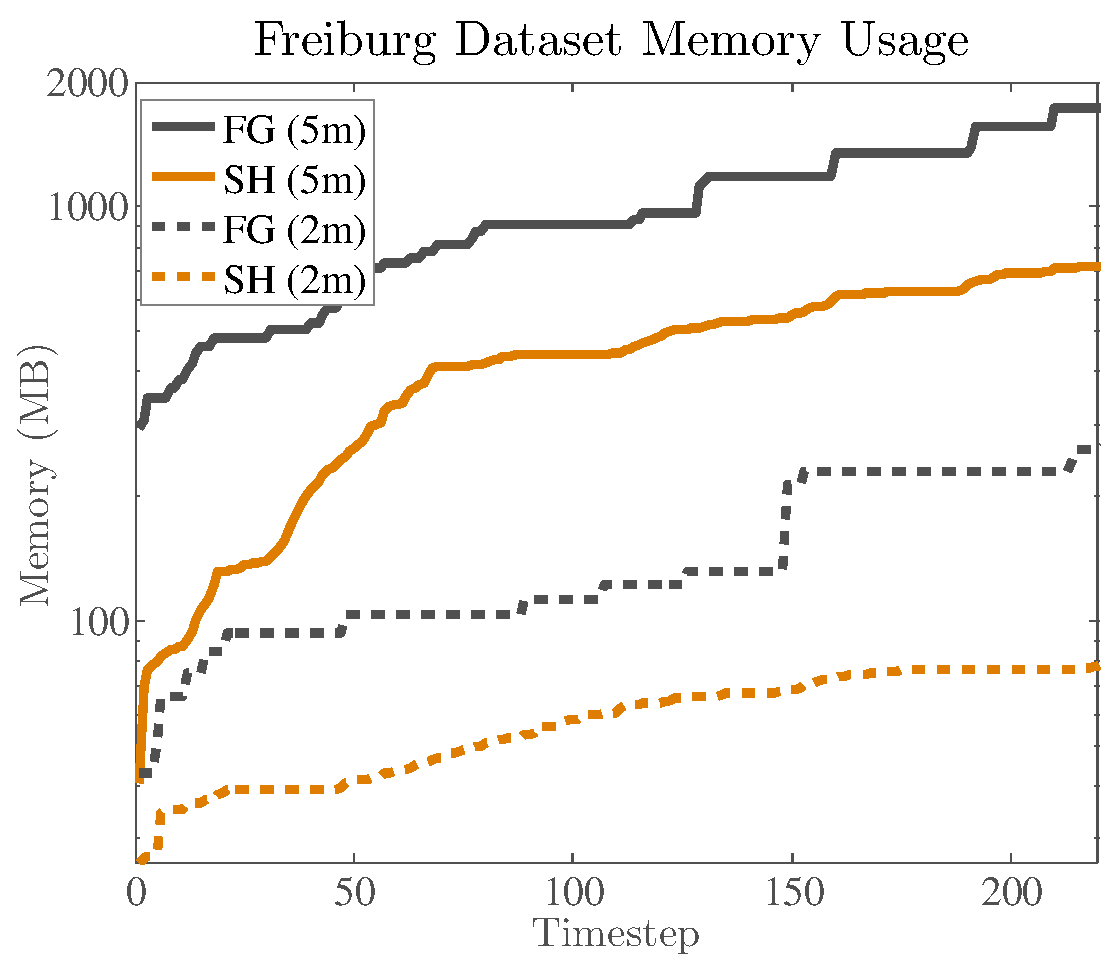
\includegraphics[width=1.0\textwidth]{img/memoryusage2.pdf}
		 \caption{} 
		 \label{fig:memory_data2}
	 \end{subfigure} 
      \caption{Depth scan iming and total memory usage over time for the
      ``dragon'' dataset (Fig.\ref{fig:dragon}). Fig. \ref{fig:timing} shows
      scan timing for 
each of the methods as recorded on a desktop computer. We compare our chunked
      approach to a na\"{\i}ve algorithm which simply allocates a monolithic
      block of volume memory for the entire space needed (Fig. \ref{fig:memory_data}).
      Memory is recorded for voxels of 3cm resolution, using both surface and
      color data. Chunks are of $16x16x16$ voxels. This figure does not account
      for the memory allocated for display meshes. We also collected memory
      usage statistics for the Freiburg \cite{FREIBURG} office dataset (Fig.
      \ref{fig:memory_data2}), varying the size of the depth frustum.}
  \label{fig:memory}
\end{figure} 

 \begin{figure}
  \centering
 \begin{subfigure}{0.475\columnwidth} \centering
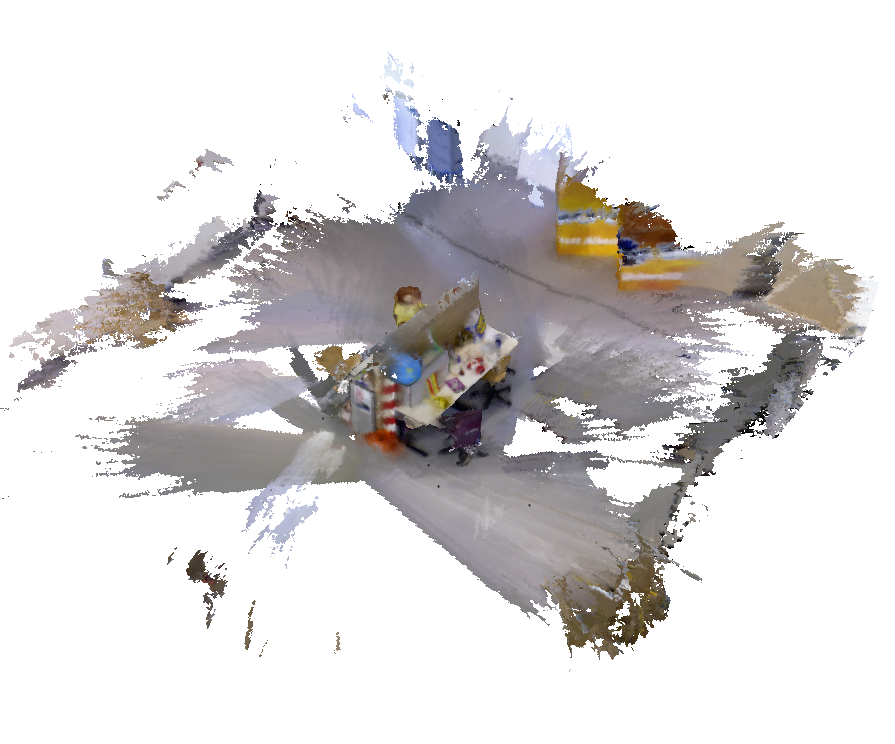
\includegraphics[width=1.0\textwidth]{img/freiburg_5m.png}
		 \caption{}
		 \label{fig:freiburg_5m}
	 \end{subfigure} 
 \begin{subfigure}{0.475\columnwidth} \centering
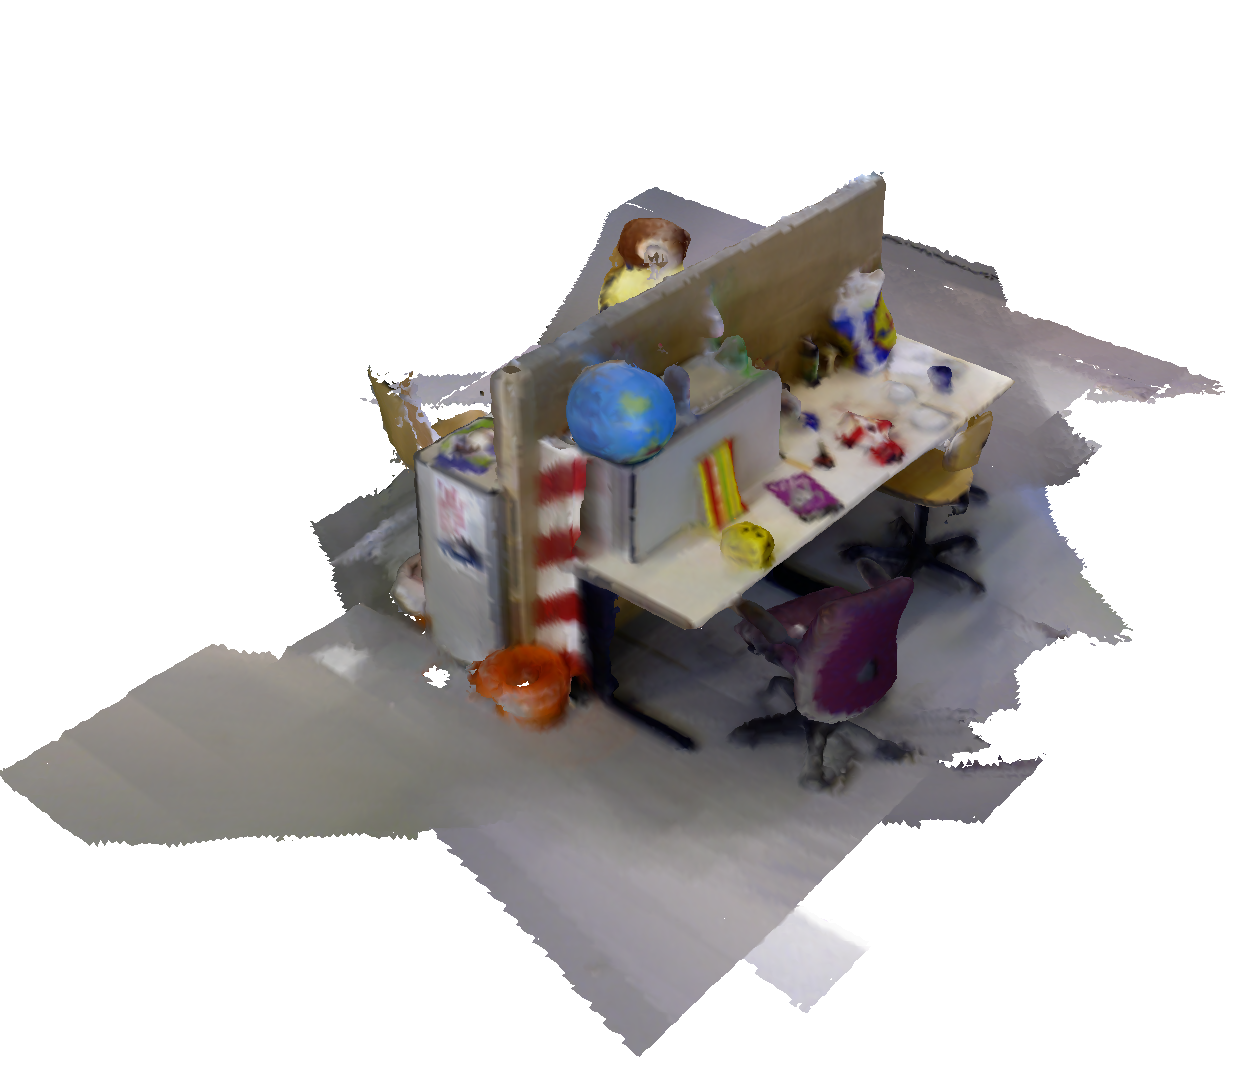
\includegraphics[width=1.0\textwidth]{img/freiburg_2m.png}
		 \caption{} 
		 \label{fig:freiburg_2m}
	 \end{subfigure}  
      \caption{Color 3D reconstructions of the Freiburg \cite{FREIBURG} office
      dataset at a resolution of 2cm. Extending the depth frustum to 5 meters
      (Fig. \ref{fig:freiburg_5m}) results in a reconstructin of the entire
      room, wheras limiting the depth frustum to 2 meters (Fig.
      \ref{fig:freiburg_2m}) limits the reconstruction to the desk scene.}
  \label{fig:freiburg}
\end{figure}
 
We implemented both the raycasting and voxel projection modes of depth scan
integration (Sec. \ref{section:scan_integration}), and compared them in terms of
speed and quality. We found that projection mapping was far more efficient than
raycasting when space carving was used (Fig. \ref{fig:timing}). However,
projection mapping results undesirable aliasing artifacts
(Fig. \ref{fig:dragon_projection_nocarve}), especially on surfaces nearly
parallel with the camera's visual axis. Aditionally, color consistency suffers
with projection carving, because rather than color being averaged by all the
rays passing through each voxel, only a single color is used for each projected
voxel center. The use of space carving drastically reduces noise artifacts,
especially around the silhouettes of objects
(\ref{fig:dragon_projection_carve}). We note that using both space carving
\emph{and} raycasting is not fast enough for real-time mapping on the device
using our approach.

\subsection{Memory Usage}
We additionally compared memory usage statistics of our chunked approach to a
na\"{\i}ve approach which allocates a single block of memory to tightly fit the
entire volume explored (Fig. \ref{fig:memory}). As the size of the space
explored increases, our approach uses about a tenth as much memory as the
na\"{\i}ve approach. This is because the majority of the space explored contains no
surfaces. Notice that in Fig. \ref{fig:memory_data}, the na\"{\i}ve approach uses
nearly 300MB of RAM wheras our approach never allocates more than 47MB of RAM
for the entire scene, which is a 15 meter long hallway.

We tested our approach on the publicly available Freiburg RGB-D dataset
\cite{FREIBURG}, which contains ground truth pose information from a motion
capture system (Fig. \ref{fig:freiburg}). In the Freiburg office dataset, a
\textit{Kinect} sensor makes a loop around a central desk scene. The room is
roughly 12 by 12 meters in area.  Memory usage statistics (Fig.
\ref{fig:memory_data2}) reveal that when all of the depth data is used
(including very far away data from the surrounding walls), a na\"{\i}ve fixed grid
approach would use nearly 2GB of memory at a 2cm resolution, wheras our
approach uses only around 700MB. When the depth frustum is cut off at 2 meters
(mapping only the desk structure without the surrounding room), our approach
uses only 50MB of memory, wheras the na\"{\i}ve approach would use nearly 300MB.

\subsection{Limitations due to Odometry Drift}
Since we do not update pose using depth data, odometry pose drift severely 
corrupts the map, especially when the same area is repeatedly scanned . We  
compare the map produced online using visual-inertial odometry to one produced
offline by first correcting the pose of the camera using bundle adjustment (a
process which takes several hours) to show the effect of drift  (Figure
\ref{fig:bundleadjust}). Double walls, accidentally carved space, and other
artifacts result when drift is present. Clearly, this limitation presents the
need for dense loop closure and alignment. High quality meshes produced using
offline bundle adjustment for pose estimates are shown in figure
(\ref{fig:apartment}).

  \begin{figure} \centering
	 \begin{subfigure} {0.49\columnwidth} \centering
		 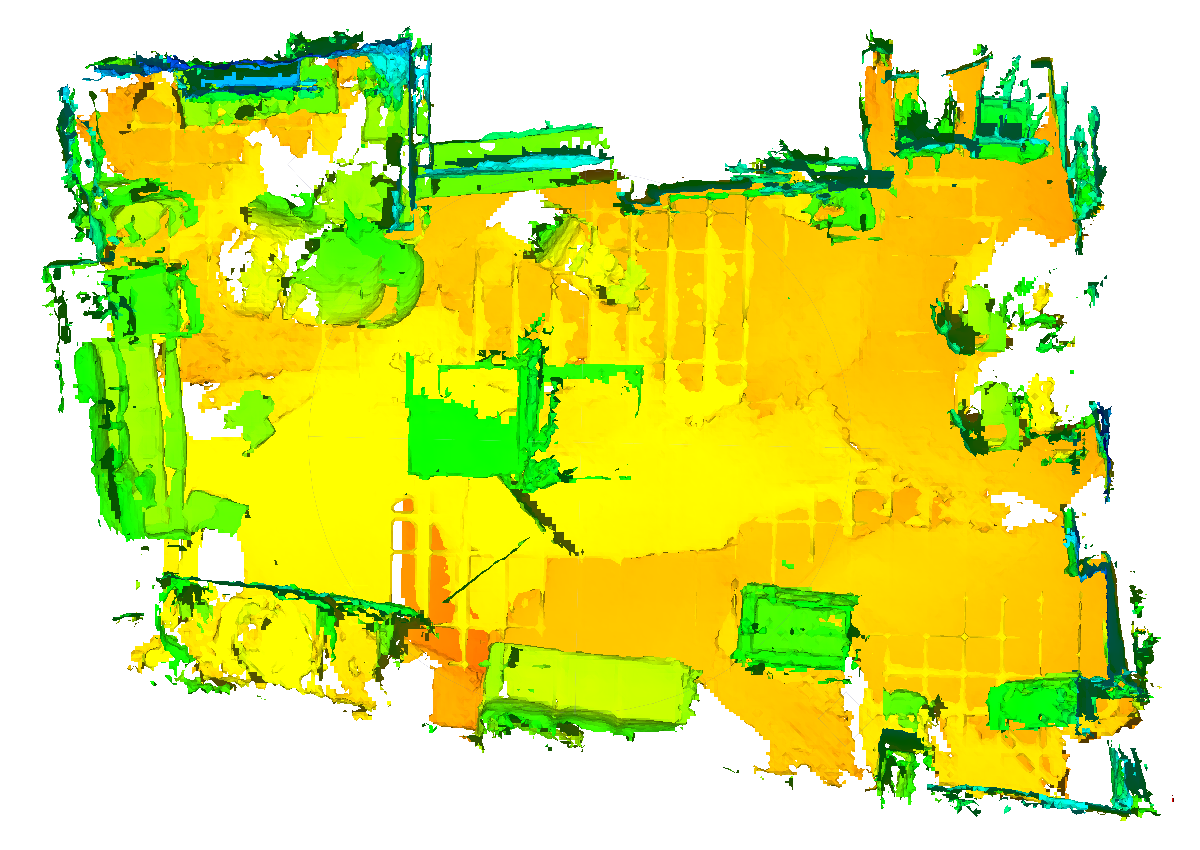
\includegraphics[width=1\textwidth]{img/gameroom_vio.png}  
		 \caption{}
		 \label{fig:gameroom_vio}
	 \end{subfigure}
	 \begin{subfigure}{0.49\columnwidth} \centering
		 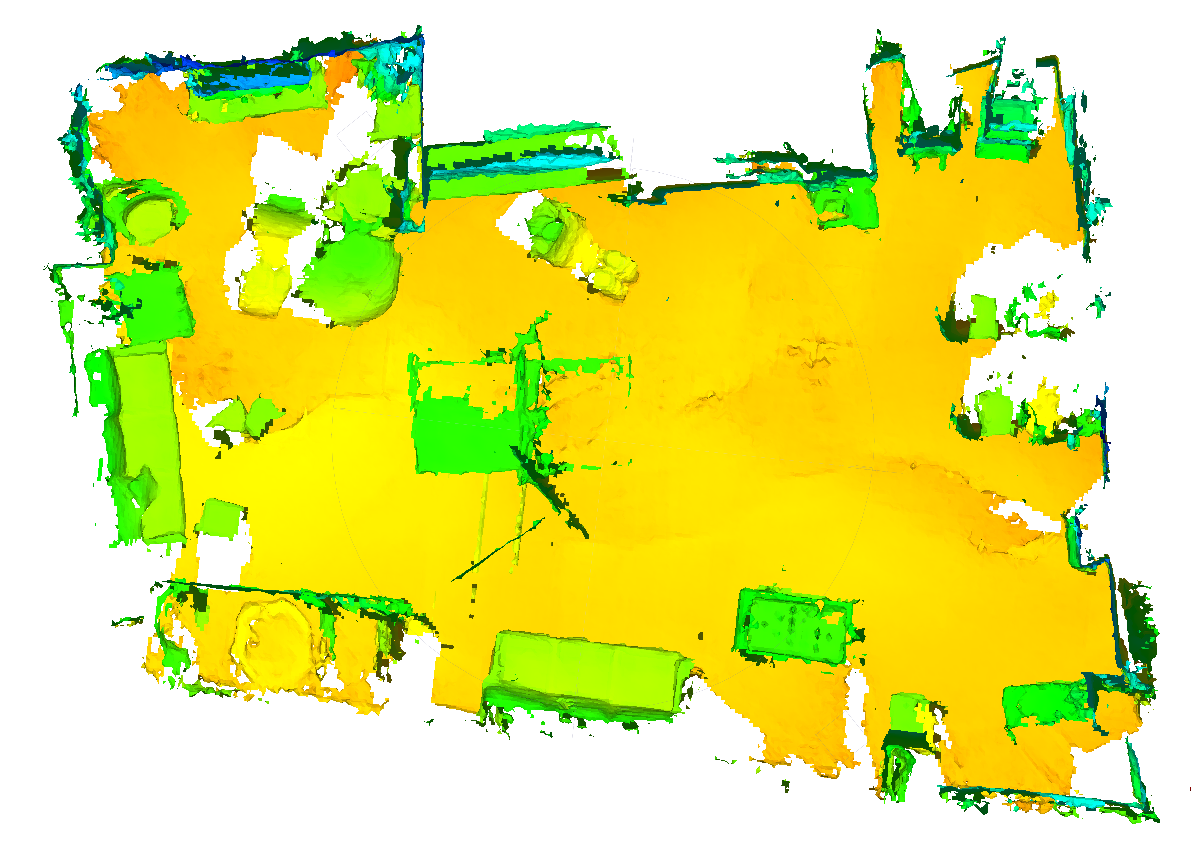
\includegraphics[width=1\textwidth]{img/gameroom_bundleadjust.png}
		 \caption{}
		 \label{fig:gameroom_bundleadjust}
	 \end{subfigure}
	 \caption{The phone device was used to scan a midsized room by walking in a
	 loop around the room three times. A top down view is shown. Meshes are colored
	 with respect to their height; the floor is orange and objects green. Drift
	 from visual-inertial odometry causes severe corruption and artifacts in the 
	 TSDF (\ref{fig:gameroom_vio}). By pre-processing the trajectory offline using
	 bundle adjustment, we can produce a much higher quality mesh using the same
	 dataset (\ref{fig:gameroom_bundleadjust}). Meshes are produced using
	 raycasting and space carving. }
	 \label{fig:bundleadjust}
 \end{figure}  
 
   \begin{figure} \centering
	 \begin{subfigure} {0.49\columnwidth} \centering
		 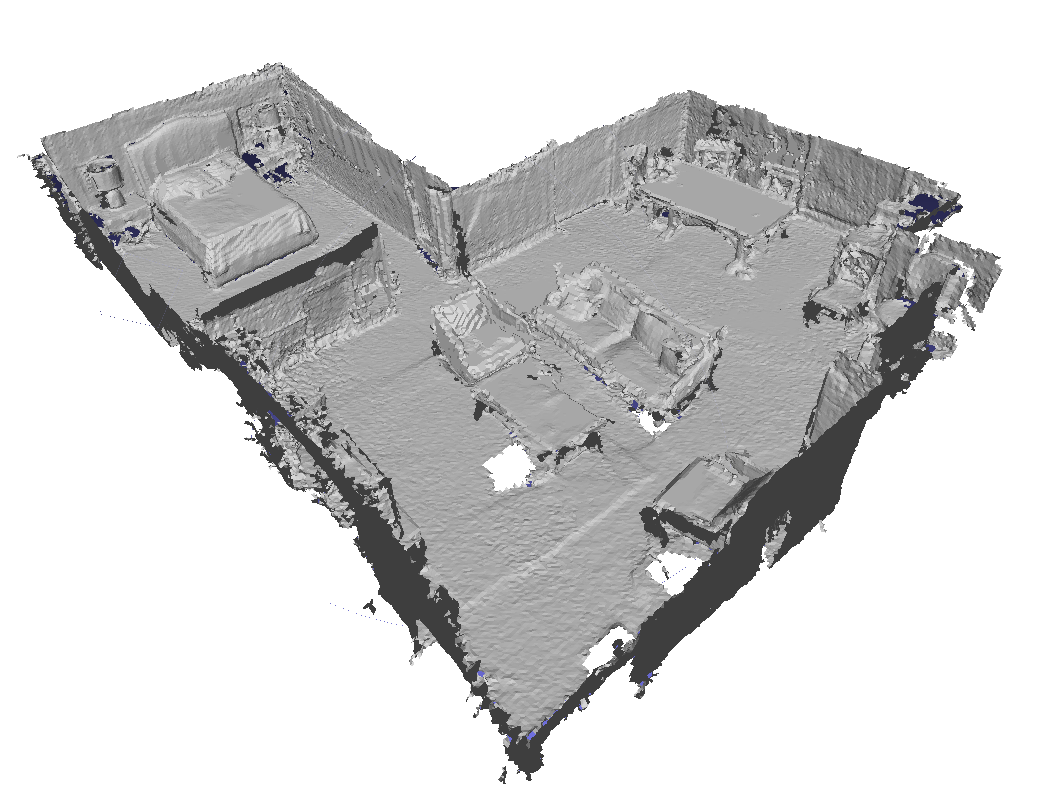
\includegraphics[width=1\textwidth]{img/apartment_scene_nocolor.png}  
		 \caption{}
		 \label{fig:aparment_nocolor}
	 \end{subfigure}
	 \begin{subfigure}{0.49\columnwidth} \centering
		 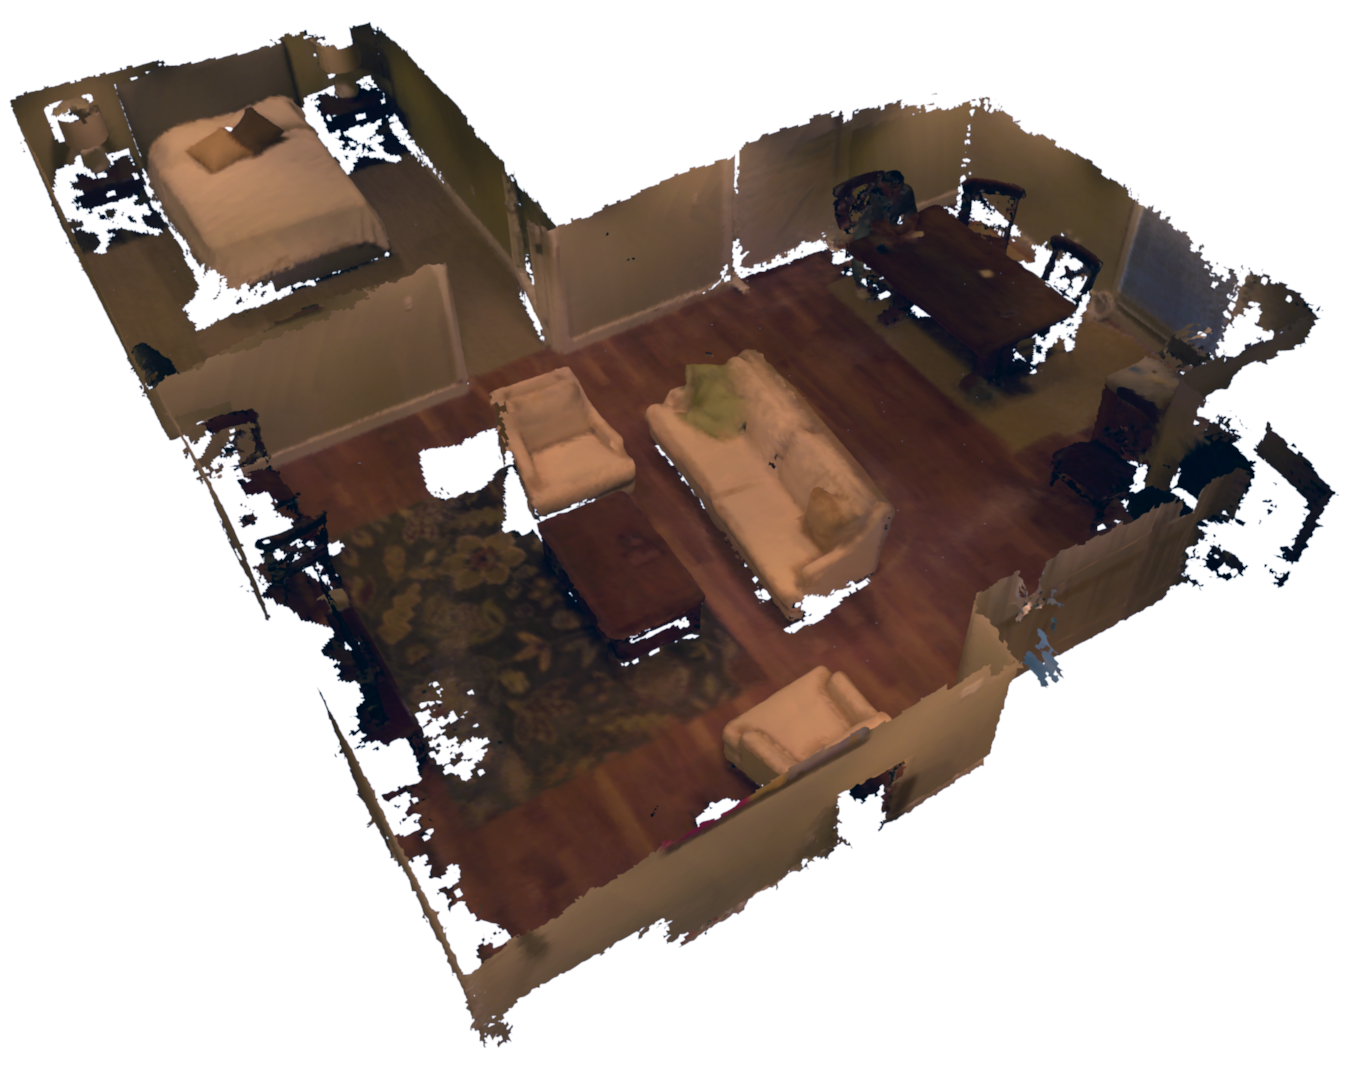
\includegraphics[width=1\textwidth]{img/apartment_scene_color.png}
		 \caption{}
		 \label{fig:apartment_color}
	 \end{subfigure}
	 \begin{subfigure} {0.49\columnwidth} \centering
		 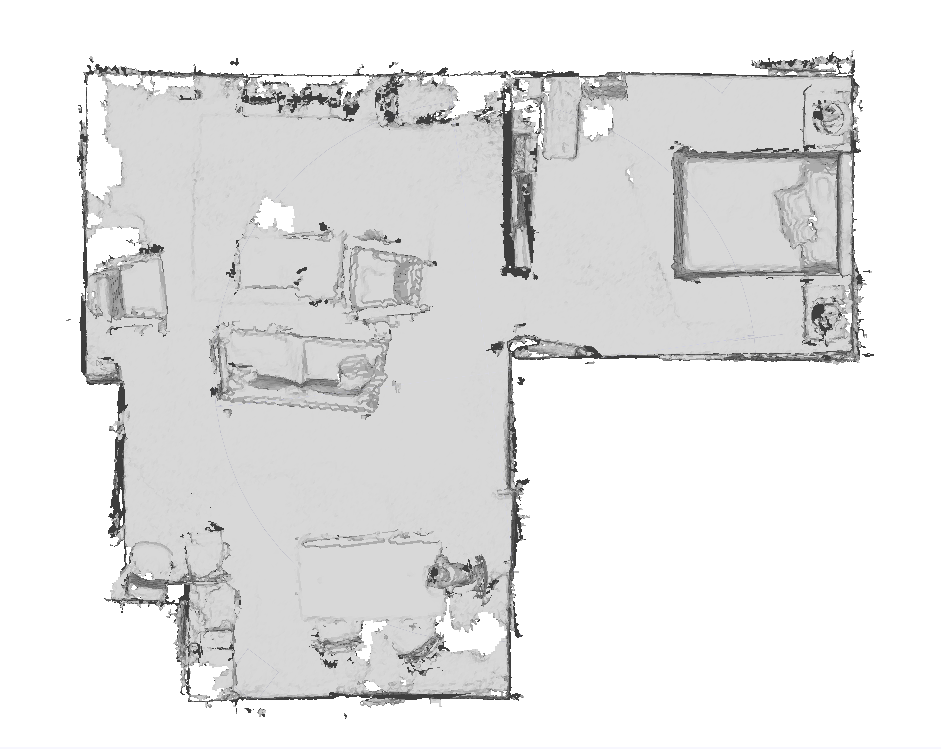
\includegraphics[width=1\textwidth]{img/apartment_scene_topdown_nocolor.png}
		 \caption{}
		 \label{apartment_scene_topdown_nocolor}
	 \end{subfigure}
	 \begin{subfigure}{0.49\columnwidth} \centering
		 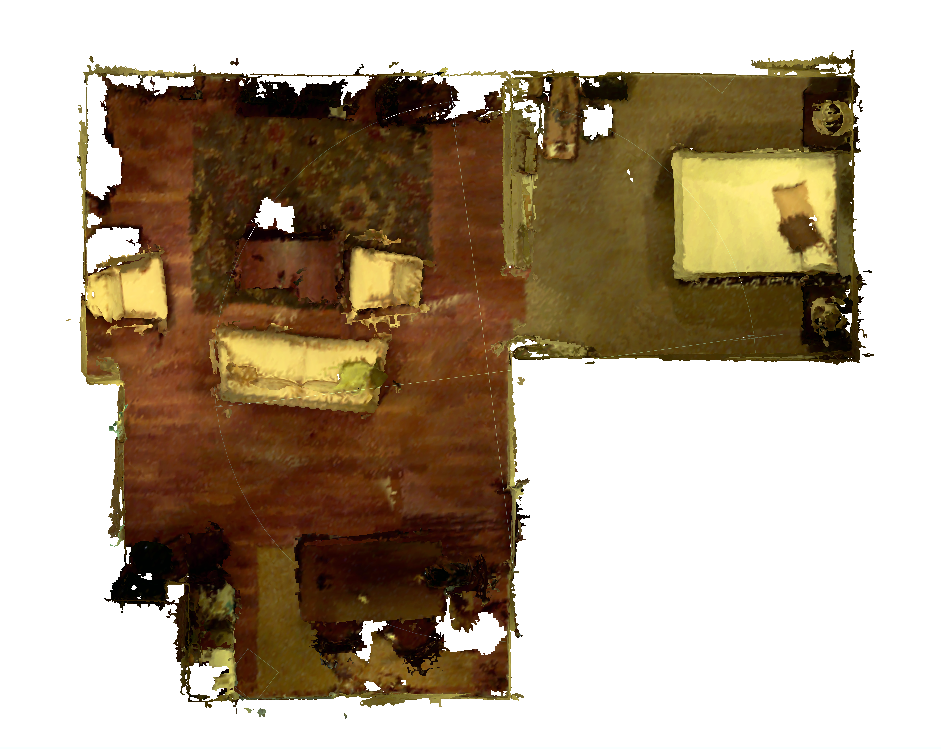
\includegraphics[width=1\textwidth]{img/apartment_scene_topdown_color.png}
		 \caption{}
		 \label{fig:apartment_scene_topdown_color}
	 \end{subfigure}
	 \begin{subfigure} {0.49\columnwidth} \centering
		 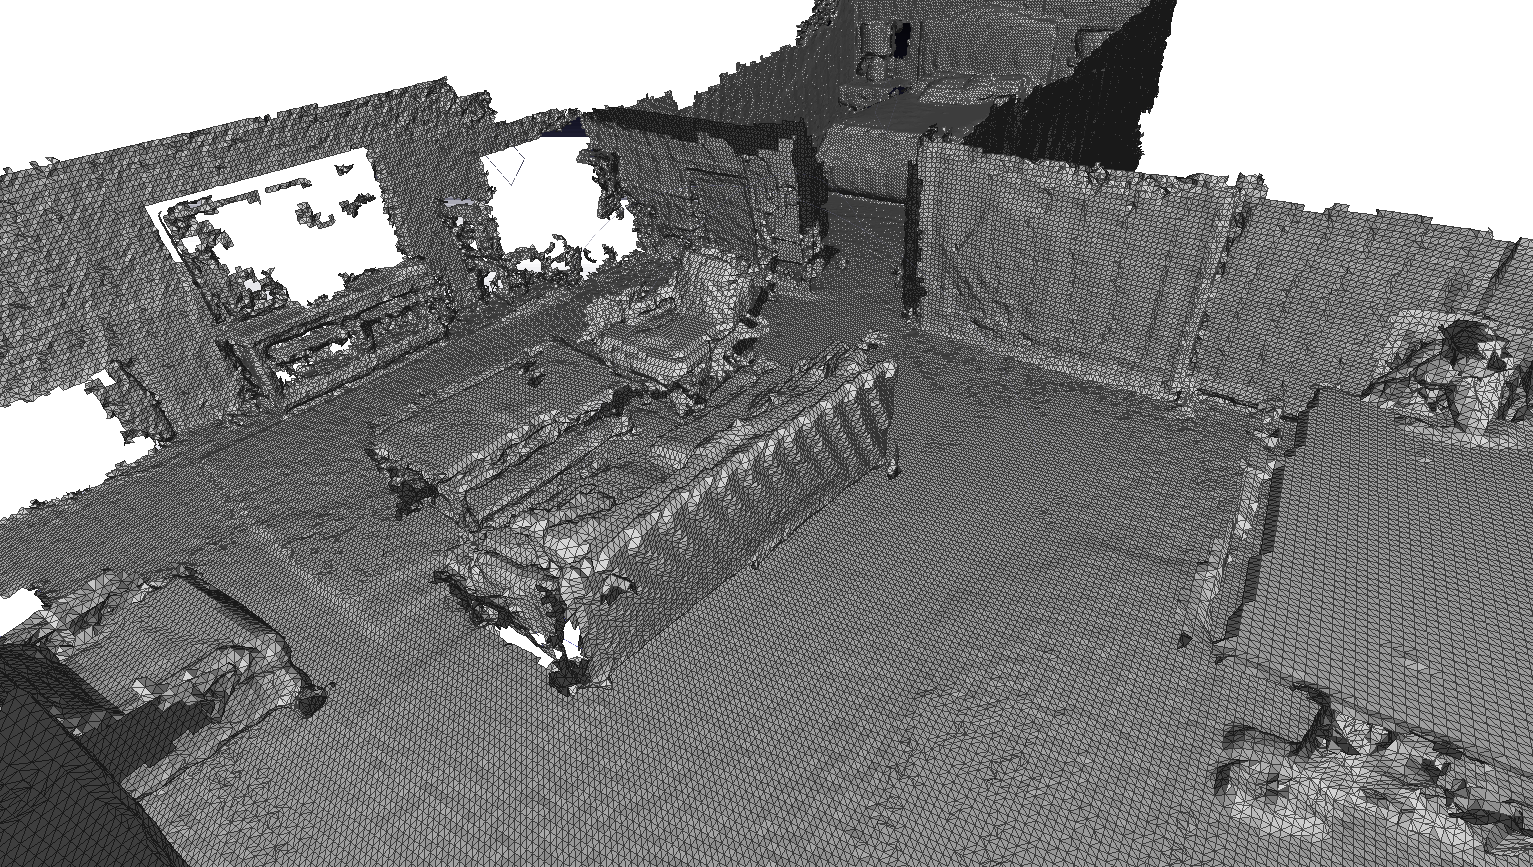
\includegraphics[width=1\textwidth]{img/apartment_scene_closeup_nocolor.png}  
		 \caption{}
		 \label{apartment_scene_topdown_nocolor}
	 \end{subfigure}
	 \begin{subfigure}{0.49\columnwidth} \centering
		 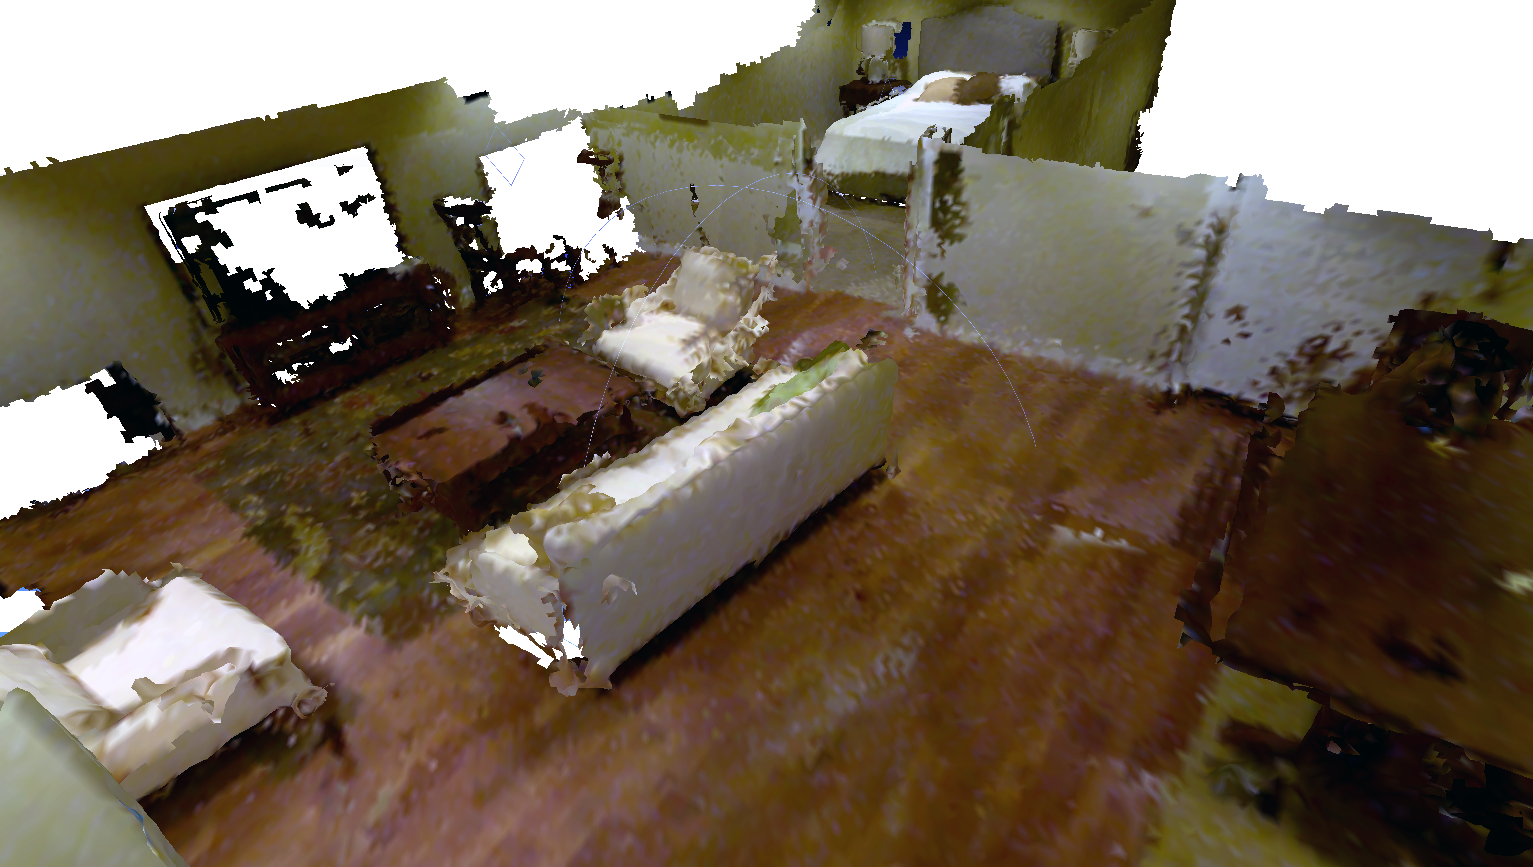
\includegraphics[width=1\textwidth]{img/apartment_scene_closeup_color.png}
		 \caption{}
		 \label{fig:apartment_scene_closeup_color}
	 \end{subfigure}
	 \caption{Several views of an apartment scene are shown without and with
	 color. These meshes were produced using the tablet device using space
	 carving, raycasting, and an offline bundle adjustment procedure to correct
	 for pose drift.}
	 \label{fig:apartment}
 \end{figure}  

%\begin{itemize}
%    \item If we're keeping around the volumetric information, what does that
    % buy us? Can it help us with loop closure?
%    \item These techniques can be used outside of the mobile context to speed
%    things up.
%    \item We gain a lot by using decoupled pose, but there needs to be a way to
 %   incorporate the VIO pose with dense alignment (like they do in Kintinuous).
%\end{itemize}
 
\section{Discussion and Future Work}
Our approach is able to create and render large-scale 3D reconstructions of
scenes in real-time using only the limited computational resources of a
\textit{Tango} device. We accomplish this without any GPGPU computing, and use
only the fixed function pipeline to render the scene. We do this out of
necessity to meet the computing requirements of a mobile device.

However, the optimizations we have made are equally applicable to other
settings beyond mobile devices. By using a dynamic spatial hash map to store
TSDF data instead of a monolithic array, much larger areas can be
reconstructed. Unlike other approaches which attempt to create large TSDF
reconstructions \cite{Whelan2013}, our approach keeps \textit{all} of the
volumetric information intact. This allows the user to re-visit locations and
improve the reconstruction.

Admittedly, our reconstructions are much lower resolution than state of the art
mapping techniques, which typically push for sub-centimeter resolution. We have
yet to see whether our approach can be combined with GPGPU solutions to deliver
large-scale, very high resolution reconstructions.One of the biggest
bottlenecks in volumetric integration algorithms is the overhead associated
with transferring data to the GPU. Because of this, all other TSDF-based
approaches (\cite{Newcombe, Whelan2013, Bylow2013, Nguyen2012}) keep only a
fixed amount of memory for the TSDF allocated on the GPU. A fruitful avenue of
future research would be in implementing the dynamic spatial hash map on the GPU
in an efficient way. 

Another area of potential research is in loop closure and pose estimation. Our
approach is purely \textit{open-loop}, taking in pose estimates from visual
odometry as \textit{a prioi} ground truth. Reconstruction can probably be
improved if dense 3D data is used to inform the pose estimator. More
importantly, a means of dealing with global pose estimation using the dense
reconstruction is neeeded. Whelan et. al \cite{WhelanLoopClose} introduced a
means of warping the mesh output by \textit{Kintinuous} consistently with global
pose updates inolving loop closures. Can a similar method be used to
\textit{directly} warp the TSDF chunk data to take loop closures into account?

Finally, there is the question of applications. What can be done with a
real-time dense 3D reconstruction on a mobile device? Applications ranging from
robot localization and planning to house-scale modelling and augmented reality
gaming are all possible.

\section*{Acknowledgements}
This work was done as part of Google's Advanced Technologies and Projects
division (ATAP) for project \emph{Tango}. Thanks to Johnny Lee, Joel Hesch, Esha
Nerurkar, and Simon Lynen and other ATAP members for their close collaboration
and support on this project. Thanks to Ryan Hickman for collecting outdoor data.
We would also like to thank Sidd Srinivasa for critique of this work.

\bibliographystyle{plain}
% argument is your BibTeX string definitions and bibliography database(s)
\bibliography{densemapping, ./densemapping} 
\end{document}
